\documentclass[onecolumn, draftclsnofoot,10pt, compsoc]{IEEEtran}
\usepackage{graphicx}
\graphicspath{ {graphics/} }
\usepackage{url}
\usepackage{setspace}
\usepackage{xcolor}
\usepackage{textcomp}
\usepackage{listings}

\usepackage{geometry}
\geometry{textheight=9.5in, textwidth=7in}

\setcounter{secnumdepth}{4}
\setlength{\parindent}{0em}
\setlength{\parskip}{1em}

\setcounter{secnumdepth}{4}
\setlength{\parindent}{0em}
\setlength{\parskip}{1em}

\lstset{
		language=C,
		keywordstyle=\bfseries\ttfamily\color[rgb]{0,0,1},
		identifierstyle=\ttfamily,
		commentstyle=\color[rgb]{0.133,0.545,0.133},
		stringstyle=\ttfamily\color[rgb]{0.627,0.126,0.941},
		showstringspaces=false,
		basicstyle=\small,
		numberstyle=\footnotesize,
		numbers=left,
		stepnumber=1,
		numbersep=10pt,
		tabsize=8,
		breaklines=true,
		prebreak = \raisebox{0ex}[0ex][0ex]{\ensuremath{\hookleftarrow}},
		breakatwhitespace=false,
		aboveskip={1.5\baselineskip},
		columns=fixed,
		upquote=true,
		extendedchars=true
}
\renewcommand{\lstlistingname}{Code Example}

% 1. Fill in these details
\def \CapstoneTeamName{		One Clock to Rule Them all}
\def \CapstoneTeamNumber{		57}
\def \GroupMemberOne{			Tasman Thenell}
\def \GroupMemberTwo{			Tristan Hari}
\def \GroupMemberThree{			Scott Metzsch}
\def \CapstoneProjectName{		One Clock to Rule Them all}
\def \CapstoneSponsorCompany{	Oregon State University}
\def \CapstoneSponsorPerson{		Dr. Victor Hsu}

% 2. Uncomment the appropriate line below so that the document type works
\def \DocType{		%Problem Statement
				%Requirements Document
				%Technology Review
				%Design Document
				Final Progress Report
				}

\newcommand{\NameSigPair}[1]{\par
\makebox[2.75in][r]{#1} \hfil 	\makebox[3.25in]{\makebox[2.25in]{\hrulefill} \hfill		\makebox[.75in]{\hrulefill}}
\par\vspace{-12pt} \textit{\tiny\noindent
\makebox[2.75in]{} \hfil		\makebox[3.25in]{\makebox[2.25in][r]{Signature} \hfill	\makebox[.75in][r]{Date}}}}
% 3. If the document is not to be signed, uncomment the RENEWcommand below
\renewcommand{\NameSigPair}[1]{#1}

%%%%%%%%%%%%%%%%%%%%%%%%%%%%%%%%%%%%%%
\begin{document}
\begin{titlepage}
    \pagenumbering{gobble}
    \begin{singlespace}
    	%\includegraphics[height=4cm]{coe_v_spot1}
        \hfill
        % 4. If you have a logo, use this includegraphics command to put it on the coversheet.
        %\includegraphics[height=4cm]{CompanyLogo}
        \par\vspace{.2in}
        \centering
        \scshape{
            \huge CS Capstone \DocType \par
            {\large\today}\par
            \vspace{.5in}
            \textbf{\Huge\CapstoneProjectName}\par
            \vfill
            {\large Prepared for}\par
            \Huge \CapstoneSponsorCompany\par
            \vspace{5pt}
            {\Large\NameSigPair{\CapstoneSponsorPerson}\par}
            {\large Prepared by }\par
            Group\CapstoneTeamNumber\par
            % 5. comment out the line below this one if you do not wish to name your team
            %\CapstoneTeamName\par
            \vspace{5pt}
            {\Large
                \NameSigPair{\GroupMemberOne}\par
                \NameSigPair{\GroupMemberTwo}\par
                \NameSigPair{\GroupMemberThree}\par
            }
            \vspace{20pt}
        }
        \begin{abstract}
        % 6. Fill in your abstract
        	The purpose of this document is to discuss the final state of the One Clock to Rule Them All project.
Included is the original version of each  development document, the changes made to these documents, and weekly development summaries for the past nine months.
In addition, this document includes project usage information and hindsight gained from development.
        \end{abstract}
    \end{singlespace}
\end{titlepage}
\newpage
\pagenumbering{arabic}
\singlespacing
\tableofcontents
% 7. uncomment this (if applicable). Consider adding a page break.
%\listoffigures
%\listoftables
\clearpage
\onehalfspacing

\section{Introduction}

The One Clock to Rule Them All project grew out of a desire to make DIY word clocks easy to build, control, and customize.
The client behind this vision was Dr. Hsu, an Oregon State research faculty working in biophysics. Outside of his research work, Dr. Hsu is a DIY electronics hobbyist.
Within the wide range of popular electronics projects is the area of timekeeping, and within those projects lies the word clock.

The idea of making a word clock isn’t a new idea.
Word clocks have existed in several forms in the past including designs that have generic displays capable of showing any word, to matrix displays of composed of predefined letters which can only show specific words.
Our client found the second layout of interest and was inspired to build one.
And this is when a difficulty arose.

There are several existing sets of code for powering word clocks already on the internet.
The difficulty is that all the existing code is built for a specific set of hardware and the software isn’t very abstracted.
For comparison, existing implementations are typically composed of several hundred lines of code.
Our finished software library can run a word clock with only around a dozen lines of code more than an empty Arduino project file.

It was this goal of making the software experience of building a wordclock less painful, more abstracted, and more user friendly that Dr. Hsu came up with this Capstone project.
Once we were placed with this project, our development roles shook down to the following: Tasman Thenell was the primary code architect, Scott Metzsch became the lead materials engineer, and Tristan Hari was the primary external interactions manager.

The other indispensable honorary member of our development team was Dr. Hsu himself.
While it was never formally set up that he would be part of the team, there were many areas of the project outside of coding where his consulting was invaluable.
While each of us brought strengths to the table around code development, Dr. Hsu was deeply knowledge about most of the other parts of our project.
Our development was greatly accelerated by picking his brain about electronics, materials, and other physical parts of development several times each quarter. Without this assistance, it is doubtful that the project would have been finished in time or achieved the same level of quality.

\section{Requirements Document}
\subsubsection{Purpose}
Historically, the clock face has had one of two display modes, analog or digital.
These formats have provided a solid mix between function and fashion, but there are many
other possible ways of visually representing the concept of time. One creative idea worth
exploring is timekeeping through words and letters. Although some examples of this already
exist in the high end fashion market, such as QWLock or others, they are well outside the
price range of an average consumer. The purpose of our project is to provide a similar
product with much cheaper production.

\subsubsection{Scope}
The name of our product is tentatively “One Clock To Rule Them All”, or “The One Clock.”
The One Clock’s function will be, simply, to tell time. However the functionality of it is
defined as being able to creatively tell time through a grid of apparently random letters.
Time will be displayed in forms such as “It is half past twelve” or “it is one fifty.” The
user will be able to set the starting time using a button component on the clock. Something
that may be assumed as a regular clock function that our clock will not do, is that this clock
 is not centered around being an alarm/scheduler device. We do not intend to have any sound
 components and thusly any alarm system will be mostly moot.

\subsubsection{Definitions}
\begin{enumerate}
  \item Time - The abstract concept that our machine is keeping track of and displaying to the user
  \item Real Time Clock - A real time clock module is the hardware component that tracks the passage
  of time regardless of the state of the rest of the system.
  \item RTC - Acronym for Real Time Clock module.
  \item Microcontroller - The brains of the clock. This module interfaces between the hardware
  components, the RTC, LEDs and buttons, and processes the logic for all clock functionality.
  This includes tasks like updating the display and processing user input from the buttons.
  \item Programmable LED - A Light Emitting Diode that has variable levels of brightness and
  color output. Each module is individually programmable in terms of brightness and color.
  \item LED - Acronym for Light Emitting Diode. Within this project, the term LED will always
  be used to refer to a programmable light emitting diode.
  \item Display - The LED lit letters of the clock face in a grid arrangement are collectively
  called the display. This term will be used to refer to the visual
  \item Software Library - The set of control software running on the microcontroller which drives all display output.
  \item User Interface - A set of buttons by which the user controls and interacts with the clock.
  \item BCD - Acronym for Binary Coded Decimal.
  \item Binary Coded Decimal - A method for encoding decimal numbers and information via binary.
  \item USB - Acronym for Universal Serial Bus.
  \item Universal Serial Bus - A communications medium by which the device is programmed and  powered.
\end{enumerate}

\subsubsection{Overview}
The following subsections of this requirements document describe product specifications as follows.
subSection 2 explains the purpose, function, and form of the product in broad terms on a less
technical level. Building on that foundation, subSection 3 breaks the functional requirements
describe in subSection 2 into technical requirements and specifications.
    Both of the following subsections are intended for conveying the entire functional
scope of the Word Clock project but at different levels. subSection 2 provides an overview of the
project while subSection 3 pertains to exact requirements which requires a more technical working
knowledge of hardware and software design.

\subsection{Overall Description}
\subsubsection{Product Perspective}
The clock we are making will be completely self contained with a battery
or wall plug being used to power the clock. There will be a microcontroller that is used to
control the LEDs on the display and interface with the RTC in order to provide accurate
timekeeping capabilities.

On the side of the clock there will be 4 buttons that will be used to set the time on the
clock and change features. Each button provides a specific function depending on the software
context. An example of this system when a basic menu is being manipulated would have two
buttons providing up and down scrolling, one button to select an option or submenu, and the
last button serving as a back or exit button.

The microcontroller will be the central piece of hardware in our clock and have the software
for running it embedded into it. The RTC will be connected to the board through 6 ports and
will be used to check the time periodically to verify that the time is still correct. The LEDs
will also be connected to the board and the microcontroller will send data to the LEDs that
tell them which LEDs to light up. Lastly the 4 buttons will be connected to the
microcontroller to set time and access additional features added to the clock.

\subsubsection{Product Functions}
Expected functionality related to standard clock features is known at this time
but other possible features have yet to be determined. A vague reference to these
future items is listed as the last function but no requirements for this item
is included in subsection 3.
\begin{enumerate}[a)]
  \item The main function of the clock will be to tell time through words displayed on the face of the
clock. Examples of the output format include “it is a quarter past twelve”, “it is a quarter to
five.”
  \item The clock shall provide a way for the user to set and edit alarms. While
  making an audible alarm isn't planned, user programmable alarms indicated by
  the display flashing are expected functionality.
  \item Additional functionality includes the possibility of adding extra features to the clock such as
color changes to tell the time of day, differences in brightness, and other features whose
development is purely contingent on time constraints.
\end{enumerate}

\subsubsection{User Characteristics}
Users of this product are expected to fall into two categories. While that might
seem to over generalize things, users break down cleanly into two categories.
The first is normal users who are just using this product as a clock. The second
type of user is the poweruser who might want to tinker with the software and
hardware of the clock in order to understand or expand upon it.
\begin{enumerate}[a)]
  \item A normal user is expected to be able to read, tell time and use a manual.
  \item Developers are expected to have the skills of a user as well as knowing the
capabilities of the hardware interfaces and the microcontroller in addition to
any skills necessary for software development.
\end{enumerate}

\subsubsection{Constraints}
The project needs to be meet a small set of physical and architectural constraints. These
constraints center around the units ability to act like a traditional clock in a reasonable
amount of space.
\begin{enumerate}[a)]
  \item The product must be accurate over the course of the year.
  \item The system needs to be compact enough to fit in a normal wall clock.
  \item Power shall be supplied via a conventional micro USB feed.
\end{enumerate}

\subsection{Specific Requirements}
\subsubsection{External Interface}
A set of 4 buttons provide the only interface to the software. These buttons
allow access to interacting with any available software menus. This is the only
point of contact between the user and the software.

\subsubsection{Functions}
The following items break down the general concepts of acting like a clock into individual
components of functionality. Together these functions are the software side of
how this product will be able to act like a clock.
\begin{enumerate}[a)]
  \item The system shall offer the user the ability to set the time via a
  physical interface.
  \item
  The system shall allow for setting, modification, and viewing of alarms.
  \item
  The system shall provide a visual indicator of an alarm going off but will not
  provide any auditory notification.
  \item
  The system shall recover from any series of inputs via the four button
  interface. Any input from other sources is considered unsupported and may result
  in undefined behavior.
  \item
  The system shall provide a menu option for switching output mode into BCD as
  well as a method for returning from BCD to the normal word output mode.
  \item
  The system shall update the time displayed every minute but the time in words
  shall be updated only every five minutes.
  \item
  The system shall provide a visual indicator for single minute increments of
  time.
\end{enumerate}

\subsubsection{Performance Requirements}
\begin{enumerate}[a)]
  \item The clock shall update the time being displayed within a second of the
  time in minutes changing.
  \item The clock shall not lose more than .432 seconds of accuracy per day.
  \item The system shall maintain this accuracy regardless of the presence of
  power for at least nine years, the lifespan of the RTC internal battery.
\end{enumerate}

\subsubsection{Physical Requirements}

\begin{enumerate}[a)]
  \item The system components, not including the clock housing, shall weigh no
  more than 5 pounds.
  \item The display shall be legible at a range of up to 10 feet for users with
  typical visual acuity, roughly equivalent to a 20/20 rating.
  \item The clock shall operate with the accuracy described in subsection 3.3.2 and
  3.3.3 within the temperature range of 0 degrees to 85 degrees fahrenheit.
  \item The grid of letters used to display the time will be no smaller than 10
  by 10 and no larger than 25 by 25 letters.
  \item The system shall be powered by a micro USB port.
  \item The system shall have four tactile buttons.
\end{enumerate}

\section{Requirements Document Changes}

\subsection{Table of Changes to Requirements Document}
\begin{center}
\begin{tabular}{| p{0.3\linewidth} | p{0.3\linewidth} | p{0.3\linewidth} |}
\hline
Requirement &
Original Requirement &
Final Product \\
\hline
Number of Buttons &
4 Buttons &
3 Buttons \\
\hline
Power Supply &
Power over USB &
Power from Barrel Adapter \\
\hline

\end{tabular}
\end{center}

\subsection{Explanation of Changes to Design Document}
There were only two significant deviations from the original set of requirements that were generated in the fall. While these changes do mean that our final product doesn’t match the letter of the requirements document, both changes were made for good reasons and didn’t result in a reduction of functionality. In actuality, one of the changes was necessary to maintain other promised functionality in the requirements.

The first change is the reduction in the number of physical buttons for controlling the clock. Our original concept for the design language of how users would interact with the clock software called for four buttons. One of these buttons, the back button, was eliminated because it was converted to a software menu option. This both simplified the hardware and made the menu interface for interacting with buttons in code more unified. This change doesn’t impact our ability to meet any other requirements that were established.

The most important change from the original requirements is how power is supplied to the clock. Keeping power delivery over USB would have been simple and this is what was in the draft requirements. During later development while working with the LEDS, we discovered that the amount of power we could pull over USB without the need for specialized hardware wouldn’t be enough to power 144 LEDS at a reasonable brightness.

A USB power supply was replaced with a traditional 5 volt barrel adaptor which powers all of the clock hardware. This also lets the user control the power draw of their project with ease. 144 LEDS at maximum brightness can draw up to 8.4 amps at 5 volts. Our version of the product shown off at Expo only supplied 4 amps so the clock was run at 45 percent brightness. The change to a barrel adaptor with a flexible range of power options was also necessary for meeting the 20 foot viewing requirement.


\section{Original Design Document}
\subsection{Scope}
This product will an improved experience for users seeking an interesting and unconventional timekeeping device.
It will provide a fashionable and affordable alternative to a class of product that is usually very expensive.
In addition to these goals, the product will also provide an opensource platform for users with the skills to modify the programming of the device.

\subsection{Purpose and Background}
The intention of this document is to breakdown the details of this project, including the steps we will take to complete it and the tools/methods we will use to effectively develop our product.
The metrics that we will use to measure product completion will also be included in this document, and will be referenced as we continue to develop throughout the year.
The background of the product arises from the personal interest of our client, Victor Hsu.
While there are similar products already on the market, QWLock by Ziegert and Funk for example, these products suffer from high prices and low avaliability.
Thses items traditional occupy a designer marker niche which doesn't allow most people to experience one.
In addition to these problems, it is also difficult to track down a model that has english lettering, as Ziegert is based in Germany.

We are not the first group of people to be inspired by the unique aesthetic and function of the word clock.
There are plenty of DIY projects online that also attempt to solve the problems of price and availability.
While these projects have been a valuable source of insight for the project, they are often very complicated and considered outside the comfort level of our expected users.
The intention of this product is to improve upon the situation by making the creation of a word clock less expensive, simpler, or both.

\subsection{Intended Audience}
The primary intended audience for this document is our client, Victor Hsu.
This document is intended to provide an approachable explanation to the project design to any inquiring individual.
That being said, it also includes enough detail to serve as a resource for individuals with low level background skills in electrical engineering or computer science who are intending on modifying the system.

\subsection{Definitions}
\begin{enumerate}[]
  \item Time - The abstract concept that our machine is keeping track of and displaying to the user
  \item Real Time Clock - A real time clock module is the hardware component that tracks the passage
  of time regardless of the state of the rest of the system.
  \item RTC - Acronym for Real Time Clock module.
  \item Microcontroller - The brains of the clock. This module interfaces between the hardware
  components, the RTC, LEDs and buttons, and processes the logic for all clock functionality.
  This includes tasks like updating the display and processing user input from the buttons.
  \item Programmable LED - A Light Emitting Diode that has variable levels of brightness and
  color output. Each module is individually programmable in terms of brightness and color.
  \item LED - Acronym for Light Emitting Diode. Within this project, the term LED will always
  be used to refer to a programmable light emitting diode.
  \item Display - The LED lit letters of the clock face in a grid arrangement are collectively
  called the display. This term will be used to refer to the visual
  \item Software Library - The set of control software running on the microcontroller which drives all display output.
  \item User Interface - A set of buttons by which the user controls and interacts with the clock.
  \item BCD - Acronym for Binary Coded Decimal.
  \item Binary Coded Decimal - A method for encoding decimal numbers and information via binary.
  \item USB - Acronym for Universal Serial Bus.
  \item Universal Serial Bus - A communications medium by which the device is programmed and  powered.
\end{enumerate}

\newpage

\subsection{Design Context}
When designing software for our clock we will be influenced heavily by the hardware components that we were given.
Our code will have subsections written specifically for use with these intended components since the microcontroller, RTC, and LED strips all have specific ways they want data transfered.
These hardware requirements will have to be taken into account if someone is using different components to create our word clock.

\subsection{Design Concerns}

For our clock the main concerns are to be able to read the clock and make sure that it is accurate and does not lose time.
We will also be concerned the clocks ability to maintain power and charge effectively.
This will of course affect the main concerns listed, but was worth mentioning on its own as it is it's own unit of the product separate from the pieces that will control readability and timekeeping.

\subsubsection{Functionality}
The time will be set through a physical interface of 4 buttons, the clock will be able to recover from any set of presses from these buttons.
Through these buttons you will be able to set a visual alarm and switch the display mode to BCD.
Also the design of the face of the clock should be able to be read from 10 feet away.

\subsection{Design Viewpoints}

We have selected three primary viewpoints from which to break down the design behind the requirements for the project.
The primary viewpoints are algorithmic, composition, and interface.
The algorithmic viewpoint was selected in order to discuss the accuracy and performance of the combination of the project hardware and our planned system software.
The composition viewpoint provides a space to describe the components of the project and how they interact, while the interface viewpoint describes user centric design components.


\subsubsection{Algorithm}
This subsection addresses some of our client's requirements about clock performance, BCD display mode, time loss per day, and the visual alarm.

\paragraph{Clock Performance}
\vspace{2mm} Design Concern: This addresses the design concern of being accurate and is primarily for the users.
The clock will need to be accurate or it is of zero worth as a clock.

\vspace{2mm} Analytical Methods: Simply comparing the clocks ability to remain accurate to another atomic based clock.
The time we have to exhaustively test this is limited and we will only at most be running 48 hour trials.

\vspace{2mm} Rationale: We decided that this viewpoint was important because it directly impacts the users experience.
Our client Victor Hsu would also consider this an important aspect as a measure of success in development of the clock.
In terms of the project Clock Performance and algorithm is entirely what determines the worth of the product, thusly making this a top priority in terms of viewing the project.

\paragraph{BCD Display Mode}
\vspace{2mm} Design Concern: This addresses the design concern of readability for the user.
Using the BCD display model is required for our project by its conception, and having the display properly lighting is paramount to the products success.

\vspace{2mm} Analytical Methods: Fortunately for this Concern, it is simply a matter of observation.
One would be required to view the clock for the entirety of a 24 hour day to exhaustively test this display, but short observation at AM PM times will be sufficient.

\vspace{2mm} Rationale: We decided that viewing the project from the BCD display perspective would be pertinent as it is what will be doing the entirety of the work for the display.
The BCD model needs to be 100\% functional for the user to read the clock, for the clock to be visible, and for the time outputs to be legible and correct.

\paragraph{Time Loss}
\vspace{2mm} Design Concern: When it comes to any solitary clock that does not sync atomically, accuracy will be lost over time due to the nature of time keeping in electronics.
This is an important concern as it once again addresses the clocks accuracy, in regards to accuracy loss over time.

\vspace{2mm} Analytical Methods: We will not have the ability to exhaustively test this, however we will be doing timing tests over short sessions to see if the time loss is accurate to the value given by the producers of the RTC.
Keyesstudio's website boasts that the clock will remain accurate within 0.1728 seconds per day, so over several days we will compare time loss with an atomic clock  and verify that the loss is within the acceptable range.

\vspace{2mm} Rationale: This viewpoint is pertinent to our project as a perspective of value of the clock.
A clock's worth is in ability to keep time accurately, and last for long periods of time.
Observing the clock from a time loss based perspective gives us an crucial outlook on the value of the end product.

\paragraph{Visual Alarm}
\vspace{2mm} Design Concern: This addresses the design concern of there being a visual alarm on the clock that does not make sound but has a visual queue that it is going off.

\vspace{2mm} Analytical Methods: Setting the alarm for a time and verifying that it goes off will be the majority of the testing required for this feature.
The test should be used after a test of the LEDs to verify that they are working correctly.
This way you can tell if a bug is caused by the LEDs or the code for the visual alarm.

\vspace{2mm} Rationale: We decided this viewpoint was important because it is a useful feature of clocks and a requirement of our product owner.
Victor Hsu was also interested in having an alarm of some type added to the clock since that is a basic function of most clocks now a days.

\subsubsection{Composition}
This subsection addresses some of our client's requirements about time loss per day, display modes, and clock controls.

\paragraph{Time Loss}
\vspace{2mm} Design Concern: This addresses the design concern of the clock being accurate over time which is important to the users.
The clock will need to be accurate and not lose the time when the clock is unplugged.

\vspace{2mm} Analytic Methods: Comparing the RTC time to the time of the microcontroller will be done every set amount of time to maintain accuracy and recover the time of the clock if there should be a power disconnect and the microcontroller loses the time.
Testing will be done though unplugging the microcontroller and then replugging the microcontroller to verify the time is still being kept.

\vspace{2mm} Rationale: This viewpoint is important to the design of the clock because it affects the easy of use and accuracy of the clock.
Victor Hsu would also consider time loss as an important aspect in the development and functionality of the clock.
In terms of time loss and composition, the RTC will be the main unit to keep time since there will not be any power interruptions with it's independent battery.
Also the RTC can then communicate the time to the microcontroller with wires so that there will always be a device keeping the time even in the event of power loss to the microcontroller.

\paragraph{Display Modes}
\vspace{2mm} Design Concern: This addresses the design concern of making the letters of the clock visible at 10 feet as well as being able to output the time in a BCD format.

\vspace{2mm} Analytics Methods: The LEDs are the main display and will allow the user to read the time based on the backlit letters on the face of the clock.
Testing will be done though a script that runs the LEDs through all colors and brightnesses as well as checking that each letter on the clock face is able to be controlled individually.

\vspace{2mm} Rationale: This viewpoint is important to the design of the clock because it affects the readability of the clock face and the letters that it is lighting.
Controlling the brightness and color of the clock will help to meet Victor's requirement that the clock should be visible from 10 feet.
These strips of LEDs will be connected to the clock through a set of wires that pass the data to the LED strips.

The other important concern being addressed is supporting BCD output mode.
Instead of powering a grid of letters, the BCD output mode is crucial for allowing the software suite to control other displays.
BCD is a generic format which could make our control software usable for a wide range of projects.
In addition to that, it also is very simple to test BCD formatting using something like a nixie tube.
\paragraph{Clock Controls}
\vspace{2mm} Design Concern: This addresses the design concern of the ability to control the clock and make changes to display settings and the time.

\vspace{2mm} Analytics Methods: The buttons will be connected to the clock through a set of wires for each clock and will be tested through pressing each button and verifying that the microcontroller gets the input.
The input types will be split in terms of a press or a hold of the button so that either can be used for possible input control.
This will test both the connection between the microcontroller and the LEDs and the LEDs themselves to make sure both are working correctly.

\vspace{2mm} Rationale: This viewpoint is important to the design of the clock because it affects the easy of use when choosing different settings for the clock LEDs or setting the time.
Victor would agree that having buttons that work and are accurate to their function is important to the design of the clock.
These buttons are the users main interface to interact with the device.
It is important that these buttons have no issues since the only other way to interact with the clock is through the microUSB port.

\subsubsection{Interface}
This subsection addresses our client's requirements about clock controls and ability to read the clock.
The interface is broken down into two perspectives: users and developers.
The user centric interface consists of a set of buttons for menu control while the developer interface consists of direct interaction with the microcontroller.
\vspace{1mm}
\paragraph{Clock Controls}

\vspace{2mm} The main design concern for clock controls was providing enough buttons for intuitive menu navigation without uneccesary complication.
A secondary design goal was to provide developers enough sources of input for any additional functionality.

\vspace{2mm} To meet these design goals, a layout of four buttons on the side of the clock has been chosen.
These buttons provide control over the planned interface scheme which is: a select button, a back button, and buttons for up and down scrolling.
An initial setup with only three buttons was considered but it did not make the interface simple enough from a user perspective.
The rational behind this was a desire to not have any button have more than one function in the core interface.
With the three button interface, that would have meant a contextual combination back and select button, or only scrolling in a single direction.

\vspace{2mm} From the developer perspective, four buttons also won out as it provides additional flexibility.
While it is not known at this time if all of these buttons will be necessary, the developer perspective is secondary to the user one.
That being said, giving additional flexibility for the physical interface for any custom project was deemed to be mostly a positive.
\vspace{1mm}
\paragraph{Clock Readability}

\vspace{2mm} While being able to control the product is important, an even larger concern was the legibility of the clock face.
The primary purpose of a clock is to provide convenient access to the time of day.
With any creative twist on timekeeping comes the concern that the creative aspects will get in the way of the core functionality.

\vspace{2mm} From the user perspective this design goal will be easy to meet.
Unlike other novel approaches to displaying time, our display doesn't require any additional thought or effort to acquire the time.
The whole idea behind a word clock is that reading the time is as simple as reading the words on the clock face.
The clockface spells out the time in words and reads like a sentence.

\vspace{2mm} While the display works very well from the user perspective for timekeeping, it comes with some large limitations for developers.
Unlike most other traditional displays, a letter based matrix is drastically lower resolution and does not use uniformly shaped pixels.
These concerns are secondary to user legibility but some choices have been made to help developers.
The current design calls for a grid which is fourteen by fourteen letters which is a larger resolution that most word clocks.
Providing a slightly higher resolution is the best we can do to help with the display of developer projects.

\vspace{1mm}
\paragraph{Developer Interface}

\vspace{2mm}
One final interface design goal was to cater to developers or users that would like to tinker with the clock software.
We would like to facilitate access to the control software without the need for expensive software tools or hardware modification.
These goals were taken into consideration when picking the board and this has lead to a flexible toolset that costs nothing.

\vspace{2mm}
This design goal has been one of the easiest to meet due to the choice of microcontroller.
The choosen controller has a standard hardware interface which comes in the form of a miniUSB port.
In addition to this, it also comes with a web based integrated developer environment which provides software developer tools with the need for downloading or purchasing software.
While most boards have accompanying software, on standard operating systems this board is plug and play and requires almost nothing in the way of drivers or additional setup.
These features of the microcontroller combined with making the default software open source should allow anyone who would like to tinker with the product or develop for it do so without much difficulty.

The other aspect of the chosen board that is conducive to development is the abundant supply of libraries and examples.
Having a product within the Arduino family of boards paves the way towards a numerous existing parts of software projects.
The process of adding hardware to the project for which there is already an Arduino library is usually as simple as including the library.
This level of software and hardware support combined with spare pins on the board should leave developers ample room for projects.

\section{Changes to Design Document}

During the course of development, several key changes were made to our original design.
Most of the changes were relatively minor and revolved around user interaction and the details of the interface.
The only major change that happened during development was moving to a different microcontroller and software platform.

This last change was made very early on in development and directly enabled the success of the project.
The initial plans called for using a very low end microcontroller board, the MPLabXPress board.
The hardware cost and software environment promised by this piece of hardware seemed in line with the project goals: inexpensive and easy to use.
While the board was cheap, the software side of things turned about to be anything but easy to use.

After several weeks of initial development and investigating getting the XPress board talking to the other components, it became clear that the documentation was very poor and that example code was lacking.
This was a newer board that hadn’t been used much for this type of project so this wasn’t very surprising.
After running into this headache, the choice was made to switch to the far more capable and proven Arduino ecosystem.
With this change, all the hardware was communicating within two days of receiving the new board.

The other deviations from the original design that are worth discussing are the changes made to the controls for the clock.
The original set of designs we came up with called for 4 buttons for ease of use: up, down, select, and back.
During development it became clear that there wasn’t a need for a hardware back button for two reasons.
Not all interfaces needed it and it could easily be replaced with a software menu option.

The second interface change came in eliminating using button press duration to indicate different things.
Once our software menu code became robust enough, any need for specialized functions controlled through long button presses was eliminated.
Maintaining a uniform control design language that relied on menus and options was determined to be more user friendly and had a lower learning curve.

The combination of these interface changes makes using the default interface more simple and makes it easier to interact with buttons via code.
The button software library handles button interaction and reduces the complexity down to a single line for asking if a button has been pressed.
This wasn’t possible when there were multiple ways of pressing the same button as described in the original design.


\section{Technology Review Document}
\subsection{Micro Controller}
The technology we are using for our micro controller is the MPBLABXpress Evaluation board.
The reason why this will be our sole selection is simply that it is what was chosen for us to use by our client.
That being said it is an excellent choice.
There are many projects that have been created using this micro controller, from things like other clocks, to home monitoring systems.
It has many pins for usage and runs very efficiently with power. The creators also provide a cloud based IDE \cite{cloudIDE} that is very easy to use and load new programs onto the board with, which is a feature exclusive to the board we are using.
A few of the competing products on the market right now is the Adafruit trinket \cite{trinket} mini micro controller, and the infamous raspberry pi \cite{pi}.
The Adafruit device is excellent as it is very small and can do all of your favorite 5v logic programs.
The only issue faced with this device in the light of our project is that it does not have enough power throughout capabilities to properly control the LED array that we will be using.
Also it would require some sort of board to be placed on, and that would lead to additional hardware needing to be bought, and potentially increasing the size past where we would have liked it.
The raspberry pi is also an excellent product. There and thousands of project examples that are out there for the pi as is.
The only reason we decided not to proceed with the raspberry pi is mainly that is more than what we need.
The raspberry pi is an entire tiny computer that can run Linux flavors and do many things.
But with that in mind, they are much more expensive as are the parts to expand the capabilities.

\subsection{RTC}
We are working to create a clock that will tell time with words instead of hands or numbers.
To keep track of the time we will be using a real time clock module that is powered by a battery to keep track of the time so that even if the clock loses power time will still be kept track of.
We will be using the RTC module to know when to update the face of the clock to show a new time.

For our project Victor has supplied us with 3 KeyeStudio DS3231 Clock Modules.
The RTC is powered by a small battery that will keep track of time even if the main power source is turned off or disconnected.
The main benefit of this clock is that is has an integrated temperature-compensating crystal oscillator and that there are pins we can attach wires to instead of having to solder each wire to the board.
In RTCs time is kept by using a small quartz crystal that has a resonance of a precise frequency.
This frequency is used to keep track of time and there can be small changed based on the temperature that the crystal is at.
In our RTC there is an adjustment made that will allow us to get more accurate time keeping when the RTC is within recommended temperatures.
Between 0 degrees Celsius and 40 degrees Celsius the clock is accurate to 2ppm \cite{ksRTC}, or in other words it will have two errors every 1 million seconds.
With this accuracy we will only lose around 0.1728 seconds per day or 63.072 per year.

An alternative to the KeyeStudio RTC is the SparkFun Real Time Clock Module.
Compared to the KeyeStudio RTC the SparkFun RTC has two main weaknesses, the first is that the clock is not have any crystal temperature correction and does not have pins to connect wires into.
Not having crystal temperature correction has main issues when you have your clock changing temperatures with the weather and seasons.
The SparkFun RTC has an advertised accuracy of 20ppm which is 10 times the errors that you have in the KeyeStudio RTC.
A 20ppm error will lead to 1.728 seconds loss over a day and 630.72 or 10 minutes 30 seconds over the course of a year.
This lack of temperature correction is a strike against the SparkFun RTC.
The second weakness of the SparkFun RTC is the lack of built in pins for connecting the RTC to the logic board.
The intent of the SparkFun RTC is to solder wires onto the RTC and then to the logic board to connect the two parts, but with SparkFun RTC being only 20mmx20mm and roughly the side of a quarter \cite{sfRTC} soldering 5 wires onto the board can be slightly difficult.
Also having pins instead of soldering wires to boards makes it easier to fix mistakes make connecting the correct wire to the correct place on the logic board.

A third option for the RTC could be the SparkFun DeadOn RTC Breakout, this RTC has some advantages over the SparkFun Real Time Clock Module but still is behind the KeyesStudio RTC in terms of ease of instillation.
The SparkFun DeadOn RTC is similar to the KeyesStudio RTC since they both have a temperature-compensated crystal oscillator to keep track of time, this reduces the error to 2ppm \cite{sfDeadOn} from 20ppm with the non-temperature-compensated SparkFun RTC.
But where the SparkFun DeadOn RTC is still behind the KeyesStudio RTC is in connectivity.
With the DeadOn RTC you still need to solder wires onto a board the size of a quarter, but instead of 5 wires there are 7 connections on the DeadOn RTC.

For our project Victor made a great choice for the RTC.
The KeyesStudio RTC is accurate, easy to connect to the board, and the cheapest of the 3 boards coming in at \$6.80 on KeyesStudio’s store page.
With the KeyesStudio RTC winning in all 3 categories that have importance to our project, (connectivity, accuracy, and price), it is the correct RTC to choose for our project.

\subsection{Fabrication Tools}
To create the case of our clock we have many tools, but the main 3 we are looking at using are a 3d printer, laser cutter, and CNC.
Each tool has its strengths and weakness that will impact our decision on what to use for all the different parts that will go into our clock.

The first tool we can use for our project is a 3d printer.
Most modern 3d printers use either ABS (Acrylonitrile Butadiene Styrene) or PLA (Polylactic Acid) which are both thermoplastics.
3d printers create objects by melting down this plastic and applying layer after layer to form the walls and internal lattice of the object.
In the settings of the 3d printers you are able to change the thickness of the walls and pattern that the machine prints for the hollow inside the object.
Both the wall thickness and internal pattern determine the strength, weight, and robustness of the object as well as increasing of decreasing the time it takes to print the object. Each 3d printer also has a limitation that comes from the size of the printing area.
We imagined our clock to be around 12 inches by 12 inches and most 3d printers would not be able to print pieces that large and if they were able to it would take a very long time to print.
3d printing can be used in our project for any parts we may need that are not easily found at a hardware store or are not flat objects.
We envision possibly using the 3d printer to help create mounting point for the micro controller, guides for LED strips, or other small parts we find cannot find at hardware stores.

The second tool we are able to use for our project is a laser cutter.
Many laser cutters use a laser beam and focus the beam to create a focus point that can melt, burn, or vaporize the material at the focus point.
The process is similar to using a magnifying glass to focus the sun onto burn objects.
Laser cutters are good for cutting acrylic, wood, and if powerful enough can cut metals.
Consumer laser cutters like the ones we have access to are usually limited to cutting plastics and woods.
Since laser cutters cut using heat and concentrated beams there is a great deal of heat generated during the process and this needs to be accounted for when choosing materials and thicknesses of materials.
Thicker materials or harder woods need to be cut at slower speeds and thus cause the material to heat up more and can leave burn marks and can warp the material you are cutting.
There is some marking techniques and cooling tools that help to reduce the amount of heat and burning that can affect the cut of a material.
We envision using a laser cutter if we want to make the housing of our clock acrylic or out of a softer or thiner pieces of wood.

The last tool that we have access to is a CNC (Computer Numerical Control) router.
CNCs use specific types of drill bits to cut materials out and create 2d or 3d shapes.
CNCs are very similar to laser cutters in their cutting process but CNCs have the benefit of generating less heat to make to remove material.
Similar to the laser cutter the cut speed depends on the hardness of the material and the speed and depth of the cut need to be adjusted accordingly.
If your material is a soft wood like pine, you will be able to have each pass of the CNC be faster and/or deeper compared to if you are a harder wood like maple or oak.
We envision using the CNC router to create the face and back of the clock.
It will be a good tool to cut out each letter on the face of the clock and for removing material from the back to isolate the light from each letter.

Each tool that we have access to can be used in our project and each has strengths and weaknesses over the other tools.
We will use either the laser cutter or CNC for most of the large pieces of the clock since they are faster than the 3d printer, and the 3d printer will be perfect for small pieces or mounting hardware of electronic components.

\subsection{Materials}
For our project we have 3 possibly types of materials to use for the case of our clock, acrylic, wood, and ABS/PLA.
Each material will have strengths and specific uses in our project.

One possible materials we can use in our clock is acrylic.
Acrylic is a plastic that you can purchase in sheets or different colors, varying thickness, and physical characteristics.
Proposed uses of acrylic are the face of the clock and case of the clock.
Side panels and the face of the clock would be easy to cut with either the laser cutter or the CNC.
We could also choose an acrylic that is opaque and this will help to isolate light from the LEDs from bleeding into other letters on the clock.
If we wanted to show off our cable management and electronics that go into our clock, transparent acrylic can be a great choice.
Acrylic can also come in mirrored sheets that can create unique ways to display the words on the face of the clock.
The one concern with using acrylic is that mounting objects to it could be a little difficult.
Mounting parts and components to an acrylic clock case would have to be done with glues since drilling and screwing into acrylic has a tendency to crack or split the material if done improperly.
Acrylic is also versatile in that we would be able to cut it with either the laser cutter of using the CNC if we find the correct bit and are careful not to crack the sheet.

Wood is another material that we have thought about using to create the case of the clock.
There are many options and choices of woods that we can choose for this project.
Cheaper or softer woods are a good choice for prototyping stage of the project since they are easier to cut and decrease the price of each prototype version. Hardwoods are a good choice for the final product because of their durability and aesthetic appeal.
The downside is that the cut time of hardwoods will be greater and the price can be more expensive compared to softer woods.
Woods will be easier to mount components into since we are able to drill into the woods with more confidence that the material will not split or crack.
Depending on the hardness of the wood we will be able to use either the laser cutter or the CNC to cut out the case of the clock.

ABS and PLA are popular thermoplastics used in filament 3d printers and can be used to print out small parts needed for our clock.
These plastics are heated up by the 3d printer, extruded, and then cool back to a solid state.
ABS filament is better when strength, flexibility, and higher temperature resistance are important to the object, while PLA has higher printing speeds, thinner layers, and sharper printed corners.
We intend to print small parts and mounting hardware for our clock so either ABS or PLA would meet the requirements we need of the part.

For the case of the clock we will be either choosing wood or acrylic for the body and face of the clock.
In both scenarios we will use a cheaper material for prototyping of the clock and then choose a more premium material for the final product.
ABS or PLA will be used for mounting hardware and any other small parts that we need to create our clock.

\subsection{Letter Grid Layout}
When looking at the grid layout there are infinite possibilities to pursue for what could be considered “optimal” or the best for our design.
That being said we will be comparing a few existing layouts for their potential of different displays.
The first one being the most popular, and one of the basis ideas for our project, the QWLock \cite{QWLock}.
The way their layout is, is to have each row with cascading potential priority in sentence structure to tell the time correctly.
So they have created in layers the exact words needed to spell out the correct time in the correct order.
Also They have whole words connected, not leaving spaces between letters.
This was a design decision to make the end product more legible but less apparently random and scattered looking while unlit.
A second grid design was one we found on an Adafruit tutorial page \cite{smallgrid} that was centered around a micro layout.
This one was only 8x8 layout, using the absolute minimum words and letters possible to communicate the time.
This was a creative design, however it loses the ability to tell time in five minute intervals, which would inherently break one of our requirements, so we will not proceed with a letter grid like this one, and will require more space than 8x8.
Another layout design was by Mike Gualtieri \cite{mikegrid}, who listed out some instructions about how to do a layout with any words of your choosing, and how to organize them in a good hierarchical fashion.
This is likely to be the method we will use to proceed, as following Mike’s “layout” algorithm is not only open source and free to apply, but allows us the freedom of word choice and layout.
The only constricting piece to this method is that it doesn’t strictly adhere by any means to letter by letter layout, or by ending in a square grid.
To achieve that may require some additional work on the method.

\subsection{Light Emitting Diodes}

One of the crucial parts of the clock is providing an interesting and legible clock face.
In order to achieve these goals, light emitting diode (LED) backlighting has been chosen to illuminate the letters of the clock face.
Using LEDs isn’t as simple as just choosing a type of light bulb, there are a strict set of requirements the final selection will have to meet.
To this end, we have selected three types of LEDs to test against the following requirements.

The LED requirements center around brightness, ease of use, flexibility, and power requirements.
The display is required to be readable at 10 feet but without using an amount of power that would require adding additional separate power supplies.
In addition, to facilitate being a programmable display, each LED needs to be separately controllable in a way that isn’t overly complicated.
Lastly, flexibility is desired as several stretch goals call for various color capabilities as well as brightness control.

The first type of LED under consideration is a small LED strip purpose built as a back light.
An example of this product can be found on Adafruit with product ID 1626. \cite{led1}
The entire module is a thin LED sandwiched in diffusing material that creates a small strip of light rather than a single distinct point.
These strips score well in power requirements, using only 20mA at around 3 volts but don’t provide many of the other desired features.
These modules don’t contain any internal brightness control, lack the ability to produce different colors, and would require the creation of a custom addressing system to allow for individual programming.

The second type of light being reviewed is a programmable RGB seven segment display (Adafruit ID 1399). \cite{led2}
These units provide several features that would be helpful for the project including flexible color and brightness.
The color capabilities are particularly intriguing because one planned feature is a having the clock face have a gradient of colors to shift through based on time of day.
The other specifications of these display units pose some of the same problems as the LED backlight described above.
While these have individual control capabilities, they require twenty one pins for a full range of control per display unit.
In addition to the complicated wiring, a separate control unit would need to be included to control these units.
Lastly, the power requirements are higher than single LED solutions because these units have seven times as many LEDs to power.

The last type of display unit under consideration is a programmable LED module.
One common example of this type of unit is the NeoPixel from Adafruit. \cite{led3}
These units provide many useful features like a unified programming interface with an internal driver which allows for full color and brightness control with a large number of pins.
One very interesting feature is the ability to tie multiple units together and control them all individually through a common bus.
Each module uses four pins to communicate with the controller.
Fully programmable brightness and red blue green color spectrum round out a tempting set of features.

The project team led to agree with the product suggestion provided by the client.
Programmable LED modules with internal drivers are the best solution for powering the clock display.
Unparalleled ease of use and flexibility fully meet the proposed feature set of the display including color schemes and variable brightness without requiring a standalone additional controller for the display lighting.
In order to get the most out of these units, the team has already acquired several samples to begin experimenting with to learn the API.

\subsection{Power Source}

Two separate avenues are being considered for powering the clock project.
The most simple approach would be a fixed permanent wall connection.
While this would work, most clocks that can function as wall clocks operate off of battery power to prevent the need for visually distracting wiring.

The final power specification isn’t yet known for the project but based on early projections and the hardware choices for LEDs and microcontroller, the target power supply needs to provide five volts at several amps.
The exact amperage isn’t known at this time due to the display resolution and subsequently the number of LEDs not yet being known.
This isn’t a primary concern as all of the following products and solutions for power have some degree of flexibility or come in multiple power ratings.

The first technology under consideration is a permanent fixed wall connection as the power supply.
Since the microcontroller and several of the best contenders for power supply regulating boards use micro USB, it would be possible to tap the existing range of micro USB wall adapters meant for charging android phones and products like the Raspberry Pi.
Exact power requirements aren’t a concern as these adapters exist in a wide range of amperage ratings and specifications.

The first potential battery based power solutions is also based on an existing range of hardware.
Like the five volt power adapters mentioned before, there exist a very wide range of five volt battery packs designed for use as portable phone chargers and universal usb power sources.
These portable battery packs come in a variety of dimensions and power capacities.
Of course these wouldn’t be the only answer for power but such packs can be charged via standard USB wall adapters which would be simple to include.

The other battery based solution being considered is to design a custom solution using an array of batteries and prebuilt voltage regulating hardware.
An example of this type of power supply setup can be seen in the BattBorg, an add on designed for the Raspberry Pi. \cite{power1}
This option would be the most flexible but would require the largest amount of hardware development to deploy.

Unlike other categories of the literature review, the only definite selection being made at this time is the use of a standard microUSB power source.
While battery power would provide an appealing feature for a wall clock, the feasibility of battery power is currently unknown as the LED arrangement and overall system power draw aren’t yet known.
Without such numbers, figuring out a battery based solution for power isn’t possible.
In addition, we have already reached an understanding with our client that battery power would be a stretch goal rather than a main focus of the project.

\subsection{Existing Software Libraries}

While the physical appearance of the clock is very important, all of the timekeeping functionality and the ability to display the time is powered by a software library running on the board.
In this case, the chosen board is an MPLAB Xpress IDE board which uses a combination of direct hardware control and c programming to control it.
Since the board supports C and C based assembly, the selection of software available is very large.
A homemade word clock has been done before many times before and we will be discussing the capabilities provided by three different software implementations of the word clock functionality.

The first version of word clock software is written in C for Ardruino by Doug Jackson and Scott Bezek.
Their software, released under the GNU General Public License, is most of a starting point than a library. \cite{software1}
This software provides nothing more than the core function of a word clock including predefined word sets and corresponding LED control, as well as simple controls for changing the time.
The library lacks any other advanced features and only drives a single color of LED.
Another setback is the almost complete lack of documentation for this software.

The second set of software under consideration is a more robust suite of clock control software from a project on the website Elektronika.
Also released under a permissive license, many additional features are included above and beyond the core clock functionality. \cite{software2}
Standout features include temperature sensor reading and temperature display support as well as a scrolling display of the date.
The other important feature of this software is a semblance of documentation.
While still sparse, the code is documented in a readable fashion.

The final set of clock software is from the QloneTwo team.
Released under the Apache license, this control software also written for Arduino is aimed at being a perfect copy of the function of the original word clock.
Nothing more than simple time support is included but an intriguing feature is strong support for button input. \cite{software3}
Other than this feature, the QloneTwo library doesn’t provide any additional functionality over the other two libraries.
This library also lacks any form of in depth documentation.

If faced with the choice of using only off the shelf existing hardware, the library from Elektronika is the most well documented and provides the most features which line up with project requirements.
Since the project focus is software design, the best course forward would be to take advantage of the useful bits of existing code under open licenses and expand it with a more flexible framework.
The core concept missing from all the software libraries that were reviewed is any ease in plugging additional features or display modes into the library.
To meet this goal and to facilitate various stretch goals, the best software choice is a new implementation based on the existing Elektronika implementation.

\subsection{Winter Term Updates}
The past term of development has led to changes in the power requirements for the project in addition to developments in terms of software support.

Power developments have centered around how much current is necessary for the lights.
Initial estimates for power requirements were high because the concept was that lights would be constantly on.
Advancements have been made in terms of controlling the lights which we have used to only ever have one light on at a time.
Because of this iterating process, the power requirements have dropped drastically to the point that a 5 volt feed at 2 amps from a power supply or USB source will be sufficient.
Because of this, battery power is still being considered for a wall mounted version of the clock.

Another major update to the project is related to software support.
The project has changed to using an Arduino board which has very broad software support.
The previous board didn't actually support any of the libraries listed above whereas the new board does.
In addition to supporting those libraries, other libraries have been found which have significantly moved the project along.
These include libraries for taking care of day light savings time and RTC control.

\subsection{Testing}
In an effort to keep things modern and hip, our team will be applying agile practices to our development cycle.
This method relies heavily on good testing practices, and with that in mind, we have a set of methods that we will use as we proceed forward.
The agile testing method we will be implementing is Lean Testing.
This in the spirit of keeping our testing accurate while not developing useless artifacts for after the project is done.
Since this is just a project and not a permanent product or company, without any further development in mind, making advanced test suites and the like are rather unnecessary.
In order to provide accurate lean testing, we will be pairing 1 team member as the tester, with two team members as developers for each unit test.
Hopefully the ones in the developer role at the time will be the ones who worked on the specific segment being tested.
This allows us to keep a very extensive testing method while we do it manually.
The project allows for this type of manual testing for most of our purposes, and the situations where we cannot manually test have been addressed in the design document.
Regarding our work schedule, we mostly will be meeting once a week, testing goals, making a week plan, and share-developing during said meetings.
This is essentially a big scrum and adds to the compatibility of our development practices going forward.

This in mind, we recognize that the Waterfall methodology is also a good fit for our project, as it seems to fall in line very well with the actual class structure.
The general steps for Waterfall are strict, and as follows: Gather document requirements, Design, Code and Unit Test, Perform system testing, Perform User acceptance testing, Fix Issues, and Deliver the product.
While this does fit very well in terms of the class structure, it falls inferior to our modified agile testing/development, due to the high variability in availability of the developers, and our client.
The clients presence is not required for the most part in Waterfall methodology, and we have decided to keep victor involved at essentially each iteration.
This of course means, our development leans much more to the modified agile style.

\section{Changes to Technology Review}
During the winter term we decided that we needed to change the microcontroller that we were using for our project.
This change came about because of road blocks and board development issues we didn't foresee when originally reviewing the product.
Here is our update to the Technology Review that we added during winter term.
\subsection{Micro Controller Winter Update}
This term we started working with our micro controller and ran into a few issues that made us rethink the choice of using this board.
The main two issues that caused us to rethink our board choice was figuring out the IDE and library support for this board.

The IDE of this board on the surface is nice because it is web based and many examples that will help with learning how to use the board.
But after further exploration we discovered many sections of code were auto generated and made is difficult for us to read and follow what was going on.

The other main issue was the library support for this board. We could not find library support for this type of board.
To get around this issue we would have had to written our own libraries or set up the existing libraries for other board types and change many defined variables and globals to what work with our board and the pins assignments on our current board.

When we ran into these issues and found little help on the internet we started to research other board options that would help us get moving forward and writing code for our project.
Arduinos were a readily available option that would be better suited for our project. We choose to use the Keyestudio's Arduino Uno R3 board because it addressed the issues with had with our old board and more.

The KeyeStudio Arduino Uno R3 runs off a ATmega328 core which has a large amount of supported libraries that would help us to easily start working with our RTC and LED strips.
The libraries we found for RTC and LED interaction were well written and had many examples and tutorials on how to get them setup and running.
The concern about the IDE was also solved with the switch to an Arduino.
We are now using the Arduino IDE which has many examples, wikis, and forums online that will help us trouble shoot issues and roadblocks that we run into when getting hardware to interact, code to compile, and flashing files onto the board.

Along with solving out two concerns with the MPBLABXpress the Arduino also brings plug and play functionality and easier ability to define and change the pins that are being used for our RTC and LED strips.
The added benefits of being able to plug in components with wires instead of soldering, ability to easily change what pins are used for communication, and addressing our concerns of the old board make the KeyeStudio Arduino Uno R3 a great choice for our new board moving forward.

\section{Weekly Blog Posts}
\subsection{Fall}
\subsubsection{Week 3}
\paragraph{Tristan}
Hello all who will read this.
Over our first week being officially on the project we were able to successfully draft out our project abstract as well as an agreement of project goals/deliverables with the client. Our Client Victor Hsu seems like a great person to be working with and is very quick to communicate and be helpful where he can. We received the Mikrocontroller boards in our first meeting with him, as well as the arduino clock module that we will be using to manage time keeping. The boards look to be a humble beginning, but before long they will turn out to be something great. Over the next few weeks Victor will be receiving some LED strips which will be doing the basic backlighting for the end product.
Overall for week one, we're just getting started so there isn't much to update, but in short it appears we've got a good team and a cool project to work on, so I'm looking forward to seeing the progress.
~Tristan
\paragraph{Taz}
Welcome to the first blog from the One clock to rule them all project. Some of the other group members have already talked about what we accomplished this past week so I wanted to take a little time to talk about our dreams for this project.

The goal for this project seems relatively simple: build a clock with a slightly unusual way of displaying time. But there is so much more beyond that. Most of our ideas are related to stretch goals and involve the idea of turning the 11x11 or 12x12 grid of letters into a pseudo screen that uses each letter as a pixel. Once we have a library of functionality to support that, the sky is really the limit.

Some initial ideas about what we could do with this:

A ticker tape style print out of the time
A ticker tape display of any custom message or associating messages with specific times
Basic games like pong
Using time formulas and the multicolor nature of the leds to make them change with the time of day
...and so much more. Already in the initial meeting our client expressed interest in all these types of theoretical functionality. Between this and the fact that everybody in the group is competent and excited about the project, I think we will end up with something great by the time expo rolls around.

~Taz
\paragraph{Scott}
Welcome to our blog for the One Clock to Rule Them All capstone project!

We will be creating a clock that will tell time using words.

This was the first week and we were able to meet our mentor/project leader Victor Hsu. He gave us each a MPLAB Express PIC16F18855 Evaluation Board to use for our clocks. The board has a IDE that you can code in similar to Eclipse in layout. I was able to run some of the basic tutorials using the LED's and turnable knob built into the board and will be trying out some other small projects with the board using LED's this week. Once we are able to get the LED strips we will be using for the clock we will be able to do more things with the board and will go through and learn about what we will need to power and connect up to our board to use the LED strips. I am looking forward to the design of the box to hold the clock and working with different materials to construct it.

~Scott
\subsubsection{Week 4}
\paragraph{Tristan}
This week was a semi productive week. We were mostly working on getting our requirements document together, and with some effort we were able to do so. For some reason, upon reviewing with the instructors we had to pretty much scrape away all of the IEEE formatting in order to get the correct formatting for this document. To say the least, this process was awful and time consuming, involving some complicated and non=intuitive syntax. I want to believe Kevin when he says LaTex is great, but this event has pushed me towards the opposing opinion. Aside from that we met with the client again and got the remaining two RTC's and some variety of LED strips. This pretty allows us to begin playing with the mikrocontroller some more. Moving forward, we'll be looking for feedback on our requirements document, attempting to fiddle with the hardware, and awaiting the next assignment!

~Tristan
\paragraph{Taz}
This past week has been a pretty slow week on the project. In the wake of feedback from McGrath, our group has started work on another revision of our Problem Statement. We consider ourselves in a reasonable position because our document was already somewhat solid.

The only large change we are still discussing is how to phrase the requirement that our clock is only expected to work if hooked up to a grid of letters that provides "enough" letters. Enough is defined as having the necessary number of copies of each letter that we can concurrently spell any of the necessary subsets of words that describe all the times in the day. This is a very abstract requirement but without it, we don't stand a chance of actually spelling out all the necessary times.

We are working to rephrase this requirement because it was are only requirement that concerned whoever reviewed our document. They were concerned that it was more of an aesthetic requirement which should be avoided because it can be hard to grade completion or satisfaction for that type of requirement.
\paragraph{Scott}
This week we received feedback on our project proposal document. We will be adding to the sections that need to be addressed and send it back to our contact, Victor to get his signature on the changed that we have made to the document. Also this week I experimented more with the board and learn a bit more about how to use the logic board that we will be using for this clock.

This next work we will be doing is on the requirements document. This project will take more time and need more feedback and more writing to complete it. This will be due this coming Friday, the 28th of October.
\subsubsection{Week 5}
\paragraph{Tristan}
Without much to report this will be a fairly bland update. This week we outlined our requirements document, and nailed down some more specifics of the end product with our client. More and more the idea of the clock is coming to fruition and i'm excited to see it come together. We also met with Jon dodge, our TA and he seems like cool dude. Other than that, we haven't had much progress to report, things are still in the early phase here and there's a lot to learn. I've been playing with the board when I can, but time is limited so perhaps next week i'll be able to explore more things in depth.
\paragraph{Taz}
The past week hasn't been all that interesting in therms of project progress. The group has continue grinding through the strict documentation requirements which is surprisingly difficult for our project. For groups with a more traditional or research oriented project, the requirements document spec works pretty well. For our project, it feels like restating the phrase "we are building a fancy clock" over and over and over...

As far as real progress is concerned, not much has changed in terms of our understanding of the hardware but we will be sitting down with the client this coming week to talk more about the lights. The strips of programmable LEDs that will power the clock face come in various spacings. We currently only have one spacing to work with but several more arrived in the mail this past week so we should be able to start experimenting with those shortly.
\paragraph{Scott}
This week we finalized our project proposal and got a signature of approval for the changes that we made. We also started and completed a draft of the Requirement Document and turned that in this Friday. We were a little unsure about how to write some of the sections and will hopefully get some feedback so we can do a better job for the final copy of the Requirements Document.

In terms of messing around with the logic board I made some more progress on using the dial to control 4 LEDs on the board to count up in binary as the dial is turned. I have a basic idea of how a demo project works to control the brightness of the LED's but I will have to look into how they use the different positions of the dial to know how bright to make the LED's.
\subsubsection{Week 6}
\paragraph{Tristan}
This week was a semi productive week. We were mostly working on getting our requirements document together, and with some effort we were able to do so. For some reason, upon reviewing with the instructors we had to pretty much scrape away all of the IEEE formatting in order to get the correct formatting for this document. To say the least, this process was awful and time consuming, involving some complicated and non=intuitive syntax. I want to believe Kevin when he says LaTex is great, but this event has pushed me towards the opposing opinion. Aside from that we met with the client again and got the remaining two RTC's and some variety of LED strips. This pretty allows us to begin playing with the mikrocontroller some more. Moving forward, we'll be looking for feedback on our requirements document, attempting to fiddle with the hardware, and awaiting the next assignment!

~Tristan
\paragraph{Taz}
Over the past week, the project has gone pretty smoothly but the documentation continues to be a slog. While we didn't face any direct problems, our project doesn't fit the normal scope of the requirements and specifications document very well. This meant that we could only use a very select subset of the 830 spec sections as most didn't fit our project very well. Even the sections we did pick still sound a little forced because our project boils down to build a clock...

In the coming week we need to finish our Gantt chart and division of tasks for the project and start the literature review. These come hand in hand since we can't allocate what needs literary review without known who is going to be in charge of categories of tasks. This wasn't done by today because of some last minute readjustments with our client on Thursday afternoon.

Our other plans for the next week include working with some new hardware that has arrived. Now each member of the group has a microcontroller, RTC, and we have some programmable LEDs to start working with. We would like to start getting these components working with each in the coming weeks.
\paragraph{Scott}
This week we finalized our requirements document. The writing of which was not terribly difficult and we were able to cover each section well. The main issue that we had was when we were compiling the LaTex file and using a .cls file to stylize the document. We had trouble getting the formatting to be correct. We eventually had to make our own style file to override sections of the class file that were incorrect. LaTex can make documents look really nice but can be a bit of a pain to format into nice formats.

This week we will be coming up with a Gantt chart because of an oversight on our part. We have talked about what we think the developing stage will be like but need to finalize dates we want to achieve different levels of progress with. The main stages we see are learning the hardware setup and powering of the clock, connecting the programmable LEDs and RTC model correctly to the board, programming the main function of the clock to output with words, and finally exploration of housing, hidden features, and LED controls.

I'm looking forward to the final stage where we get to work more on the design of the housing and hidden features. The sky is the limit on the extra features we can add to our clock. It will be fun to experiment and create cool features for our clock. I plan on spending a lot of time tinkering and creating features for the clock.
\subsubsection{Week 7}
\paragraph{Tristan}
This week was mainly an uneventful once again, we spent a lot more time than we should have on our technical document due to some confusion about the assignment requirements. The issue was that we thought the format had to 100\% match the example document we were given, due to some of the wording of the assignment and what kevin said in class. That being said, after struggling for hours we finally got it done and brought it to Jon for review, where he promptly told us we didn't have to do any of that, and we were exasperated to say the least. That being said, as a group we've gained some more TeX knowledge that I'm sure will come in handy down the road. Other than that we haven't done much, we finished up our tech review portions and are piecing it together for monday, and looking forward to working with some of the coding in the next few weeks!

~Tristan
\paragraph{Taz}
During the past week the team has started doing the first phase of long term planning and serious design for the project. We hadn't finished our Gantt chart with the Requirements and Specifications document but we completed it this week as part of planning our topics for the lit reviews. In creating the chart, it quickly became apparent that this would be a very rough estimation of our division of labor. While we would like to be able to move forward with a better estimate, it isn't really possible to know how long some of these tasks will take until farther down the road.

The next phase of the project centers on the last large pieces of documentation due this term. The next immediate ones are the literature review, and the progress report. Out of these two, the more interesting one will probably be the literature review as it will allow us to actually start working with the concepts of our project more closely.

When dividing up the topics for literature reviews, we took special care to ensure that each team member got 1 topic from each area of our project: internal hardware, external hardware, and software. This way everybody would be involved in all the parts of the project. We felt this was necessary because there are some phases that, according to our Gantt chart, the only tasks available will be from one area. For example, at the beginning, all the tasks are about getting to know the hardware and getting it to communicate.
\paragraph{Scott}
This week we worked on the Technology Review for out project and our review was a bit different than most. Victor had supplied us with micro controllers, LED strips, and RTCs so we did not have to make a decision on which to use, but instead researched how these parts compared to alternatives made by other companies and vendors. I was in charge of researching about the RTC, material choice for our clock case, and the tools we can use for fabricating our clock case.

For the RTC we were supplied with a KeyesStudio RTC that, after some research, was a great choice by Victor. The RTC has temperature compensating crystal oscillator to bring the error rate of the RTC down to 2ppm, pins for easy connectivity, and is the cheapest temperature compensating RTC I could find online. All these characteristics make the KeyesStudio RTC the correct choice for our project.

For the materials and fabrication tools for creating the clock case we were able to choose what we wanted to use. We are thinking about using the CNC and laser cutter for most of our components and maybe the 3d printer for smaller parts we are not able to purchase. The final case will be made out of a combination of wood and acrylic or out of all wood.
\subsubsection{Week 8}
\paragraph{Tristan}
This week was pretty laid back, we got our assignment done nice and early, and there wasn't much problems there. There was a little confusion with the manner in which we merged our individual contributions to this document however. Everyone did their part excellently well and in a timely manner, but attempting to merge our individual pieces cause some unfortunate splicing issues and we had to manually resolve those. Aside from that, all we really did this week was meet with out TA Jon, who as always was a pleasure to speak with and had some helpful insight about our current and future work for the term. Moving forward, we're awaiting feed back on our technical review and waiting for the next assignment!

~Tristan
\paragraph{Taz}
The majority of the work that took place this week occurred in a frenetic burst of activity on Monday. The tech review wasn't very difficult for our project but in some ways, it also wasn't very technical. The majority of topics we needed to look into and do research on were hardware related and so it was less of a literature review and more about writing about finding the three best looking components for the job. A large portion of the work is still programming but since nobody on the team has extensive experience with hardware, we had a lot more research to do in that department.

Despite these challenges of fitting our slightly unusual project into the generic framework provided for this paper, we didn't have much of a problem completing it. As always, procrastination is always a bit of problem in the group but we had something presentable by midnight with everybody having contributed three sections. For the last two documents, I would love it if the group could get started earlier.

Moving forward, the last major material to write for the term is the design paper. The only challenge I anticipate for our group is that we still need to figure out a bunch of hardware choices and learn about how these pieces of hardware interact. Since we can't do this until we have the hardware, there is small chance some of the choices we make to put into our design just won't work.
\paragraph{Scott}
This week was not very eventful and the main project that we worked on was the tech review. We had a bit of an issue getting citations to correctly display in our latex file, but found a solution after a bit of time on google. Past working on the Tech review we met with out TA to get some feedback on past assignments.

We will be busy next week working on the design document and the progress report paper and recorded presentation. We will probably use OBS to record the presentation since it is free and easy to work with. This next week will filled with working on projects and papers for this class and others.
\subsubsection{Week 9}
\paragraph{Tristan}
There wasn't much done this week as far as actual progress goes, we're still kind of early along (despite being at the end of the first term) but we got some progress report planned out so there's that. Moving forward from here, we really want to plan on tackling the harder aspect of this project, which is the electronic and hardware components. None of us have really done that kind of thing before, at least to this scale. So what we really want to do to ensure the proof of concept is to get all the hardware components communicating with eachother. That's kind of the next step. Vague, but definitely measurable.

\paragraph{Taz}
In the past week, we haven't done much other than planning related to our design document writeup. While this has been somewhat productive, the work we really need to have a more solid plan for the project hasn't really been done yet and likely won't be done until people get less busy when the term ends.

The current problem with this project is that it is very hardware dependent and as CS people, we don't know the hardware details already and doing research for the lit review was only so helpful. We really just need to be getting all the hardware to communicate and get that portion of development out of the way. Building any sort of plan and timeline of development without knowing about the inevitable pitfalls of hardware development we might encounter is slightly pointless.

Not to make things sound completely negative, the project will probably end up fine. The flow of necessary work for our project and this term didn't fit very well with the typical document process that was set out for this term. That being said, we should be able to turn in a complete design document although our ability to follow it in the future might be less than some other groups.
\paragraph{Scott}
This week we didn't make much progress on our design document with the holiday and short week. We met with our TA and got some feedback on our tech review and some information about the process and requirements for the progress report. We plan on making more headway in both our design document and progress report this week now that everyone is back in Corvallis and able to meet up easier.
\subsubsection{Week 10}
\paragraph{Tristan}
This week was mostly spent hustling through the end of some difficult classes for the majority of us. That being said, we also spent some time doing the design document. I know I can speak for myself and a lot of other students when I say we found this document to be less than intuitive to beign to completion. We didn't find the instructions to be clear enough so me and my group spent a lot of time asking our TA and Dr.Winters about what is actually t o be expected. After visiting Dr.Winters' office I was able to find some examples and produce what we believe to be a decent copy. We are awaiting feedback on this document now.

Moving forward, it's the end of the term so I believe the only thing we have left to do is our video. This should be pretty fun, but with that in mind we've had almost no discussion about how we are going to proceed with that. Personally I'd prefer a live video with a whiteboard over talking over a powerpoint, but I am willing to work with whatever the group would like to do in the end.
\paragraph{Taz}
The final week of work on Capstone documentation has been a real drag. While none of the individual assignments are very difficult, the grading is nebulous and the specification for the Design document proved to be a terrible fit for our slightly unique project. We spent four days as a team this week trying to figure out how to cram our loose set of requirements and very not-finalized ideas into a concrete design for the project.

The difficulty with this document wasn't for lack of trying to make progress. We sought out more outside help for this assignment than we have with any other project for the class and still felt terrible about it by the time we turned it in. Our TA provided some information which was enough to get started but fitting our project into viewpoints went terribly. We also met with Winters and got to see an example but this also wasn't very helpful.

Going forward, this just leaves us with one final assignment, the progress update. Other than the slightly inane requirements imposed upon the format and method of delivery, we aren't worried about it. McGrath, what did Google Docs/slides do to offend you to such an extent? Is the slight reduction in visual quality (emphasis on slight) really more important than the features it provides as a real-time collaborative tool and the ease of use?

Ranting aside, working through these last two documents has felt very frustrating. I know the documents are supposed to be the how of the project but for our project, which has a very large amount of hardware overhead before we get to do any programming, we really have no idea what we are doing yet. Our last few documents have been very vague because as CS people, we really have no clue about how we are going to put the hardware together and get it all talking so the rest is pie in the sky until we have time to actually do this. Between other classes, large amounts of unhelpful writing for this class, and real life, none of us has had that time. All in all a very frustrating way to end the term.
\paragraph{Scott}
This is the final weekly update for the fall term of 2016. During this week we finished working on our design document and began work on our progress report that will be due this week. Thankfully Taz has some video editing experience in the past which will make putting the presentation video together easy, now all we need to do is create content for the slide show that is going with the presentation and write out report on what we have been doing for the term. Once we are done with both of those we will be moving on to winter break and will come back and start the process of writing code and getting out clock to display the time with words.

Happy Holidays!

See ya in 2017!
\subsection{Winter}
\subsubsection{Week 1}
\paragraph{Tristan}
We're at the point now where we've got a basic understanding of how the hardware components are going to work with one another, we just need to grind our way through the knowledge barrier involved there. What really needs to happen at this point is to just clock out (hehe) the software work. It's all doable, we have a design in mind, and we've tested some libraries that we will use. Going forward, this will be what we do. We are potentially reviewing the microcontroller that we're using as well.

\paragraph{Taz}
The clock project is going along fine but we really need to step up our programming development. The initial hardware hurdles are proving annoying to get past and none of us really has the skills to easily take on the remaining hardware setup steps. Once we muddle through this step, we can move on fully to software development.

One of the first concerns from the software perspective is figuring out the capabilities of this microcontroller. It should be fast enough to power the core requirements, powering the clockface to show time, but past that, we need to figure out if it is fast enough to support some of the stretch goals. In the standard operating modes, we have a whole minute to get ready for the next update, but some of our other goals entail powering some kind of actual frame rate.
\paragraph{Scott}
From a coding standpoint we are a bit behind the curve on this project. The main hurdle that is stopping us from writing code for our project is finding information and reading how to work with our board. When we first looked into the board we found example code that seemed straight forward, but then after we did more research into tasks we would be doing and there were little to no examples that I could find. Also looking into the example code and we found that much of it is auto generated by the IDE and was difficult to write and understand on our own. We are going to do more research into how we can accomplish our project with this board.
\subsubsection{Week 2}
\paragraph{Tristan}
Well, this week we started getting more into heavy development and cracking away at our actual build. In a good and bad manner, we progressed enough to find some details about our project that we were certainly going to have to work out. As it turns out, the MBPLAB board is a very quality board, and definitely has the potential to get the project done as we had initially found. However, the immense amount of overhead and effort required to get that board working as we would expect has lead to us to the conclusion of using another board. This was not a decision made lightly by any means, we spent many hours verifying and researching the one we have decided to move forward with. The alternative (name slipping my mind) is at exactly the same price point, but provides better functionality, libraries, and pin support for our project. We will be updating our client this week, with the changes we have in mind. This is a good thing in terms of progress, im looking forward to the results this week.
\paragraph{Taz}
In the past week of development, not much has changed from the previous week. We face the same issues that have been holding us back which mainly center around hardware power problems. Getting everything powered isn't completely stopping us but it will prevent us from testing full led grid implementations until things can be fixed.

One hope for all this is that we are having a work session on Monday which should get us to the point where we can narrow down what hardware we need and how best to acquire it. Another goal for this session is to setup basic communication with several of the LEDs in a small enough configuration that we can power them straight from the 5 volt output of the microcontroller. While it isn't much for progress, at least weekly meetings are starting to happen which should help move things along.
\paragraph{Scott}
This week we didn't make much progress researching how to get our board up and running. I am having arm surgery up in Portland to remove a plate from my arm. We will work more on this next week when everyone is back together and not on pain meds.
\subsubsection{Week 3}
\paragraph{Tristan}
This week was a good one in terms of progress for our project, we were able to finally get accurate time readings from the RTC! This is very exciting, and using the library we have moving forward, this meets perfectly with how we'd like our project to be in terms of approachability. The code so far is VERY understandable and easily changeable without causing a spaghetti salmagundi. I'm very excited for next week because our goal will be to power the LED's and get changing lights based off of time values being read. If we can do that, weve essentially built the structure for the rest of the project, and the remaining software development is just essentially filling in the blanks. Woohoo go team. I missed this weeks meeting with Jon Dodge due to an interview, however my teammates filled me in on the updates and things to be moving along well. We our meeting again with our client next week, at his earliest convenience to update him on the progress.
\paragraph{Taz}
This week has brought with it some massive changes to the project. Development had been stalled by an inability to find documentation about getting the hardware to work together or how to communicate with it in code. After one final sweep for any documentation we may have missed earlier in the project, we have decided to give up on this board.

After weeks of frustration and minimal progress, this decision was very refreshing. Our research led us to an inexpensive Arduino Uno clone which keeps within the same goals that Victor had for the project: inexpensive, easy to develop for, accessible. The Uno board manages these things by also having a web IDE, coming with a wealth of documentation and hardware support libraries, and only costing around 10 dollars.

While we probably should have figured out a change like this much earlier in the term, I'm hopeful that this will put us back on track for the overall project.
\paragraph{Scott}
This week we came to the conclusion that the current board we have will not be practical for our project. The main reason is that we will not be able to use this board is because of the learning overhead to get the board running and control the different pins will be too much of a time commitment for us to finish the project in a reasonable time.

We have purchased a Keyestudio Arduino Uno in replacement of the board. We choose this board because there are lots of tutorials, wiki's, and forums of information on the web. During this week we were also able to get the RTC to communicate with the board to print in the serial monitor. We realized that soldering the parts together was a bit difficult because of the size of the pins and small distance apart. To fix this issue we have purchased a set of 40 wires with a male pin connection on one side and a female on the other. This will help to let us plug in components as we need them.

We will need to set up a meeting with Victor to tell him about the changes to the board and show him what our progress has been so far.
\subsubsection{Week 4}
\paragraph{Tristan}
This week we made some awesome progress. We got several fun libraries rollin, we've got consistent reads from the RTC, were got Lights rollin' deep. It's awesome. We've set up a meeting with victor for next week now that we have solid progress to talk about our current status and what we'll need to move forward. We're gonna be needing buttons and an additional power source, but I have absolutely no doubt that he will provide as we've talked about this in the past. Basically moving forward we need to develop our time library, which should be fun!
\paragraph{Taz}
Over the past week we have accomplished more hardware progress than during the entire rest of the project. Switching to a board with better support and documentation payed off in a massive way and we've already been able to get more hardware communication going on than we even came close to with the old board.

Resources that have proved very helpful include the AdaFruit LED library which got us up and running with lights in a matter of minutes. In my mind this is how easy it should be to get this kind of simple hardware running. More importantly, this is exactly what our client had in mind in terms of ease of use so that others can use what we write for this project.

For next week we are going to try to get the RTC time set and be able to read the time as well as perhaps a way of displaying a condensed version of the time or date on a few LEDs. While this isn't a great product demo, it would probably suffice for a midterm progress update.
\paragraph{Scott}
This is we have made more progress getting all our components working together and talking. We have found and implemented some libraries that will help with RTC and LED communication. We also successfully learned to control the LEDs and have them cycling through the rainbow. This is a big step for our project since these are the two main pieces that make up the clock and we have them both working.

Then next steps will be to take data from the RTC and display it in some format on the LEDs. We will start out with something simple and portable using a strip of LEDs, but once we have the logic down we will move on to making grids and soldering strips of LEDs together to form the matrix of our clock face. Another goal we have for next week is to start designing the layout of the words on the clock face using tools we have found online. The last thing we have to do is finish up the progress report and video and submit those. Next week should be busy.
\subsubsection{Week 5}
\paragraph{Tristan}
This week was a fun one. We finally had our meeting and settled with victor exactly what we wanted to buy in the spirit of production of the end product. We settled on some awesome looking buttons that have lights of their own and are made of metal. They look sweet. Also we worked on combining the RTC code with what we have rolling on the LED time code. It's a bit of a trick but things are coming a long well. We are working on getting everyone set up with usable strips for individual progression. The other trick is to figure out how we're going to power all the LEDs. Victor is getting additional power units for us to use but we will have to wait for those to arrive likely before we can get the LEDs fully working. Next week should be fun!
\paragraph{Taz}
During the past week significant software progress has been made. Not only is using the new board been going smoothly, we also showed it to Victor for the first time and got his approval on the hardware. The highlights of that meeting were where we are going next with the project and getting some new hardware ordered (power supply, watch batteries, buttons).

On the software side of things, we have figured out a few more capabilities of our LED software library. The LED's can now be run with only one light on at a time which means that power isn't an immediate concern for testing. This won't be usable in the long run because it relies on the code being simple enough to run almost instantly but it works for testing with only a few LEDs. In addition to that, Tristan figured out how to set the time on the RTC, read the time from the RTC, and setup alarms.

We need to look into using hardware interrupt driven alarms as a means of idling the microcontroller going forward.
\paragraph{Scott}
This week we figured out more about connecting out RTC and LEDs to the Arduino. We have the ability to read data from the RTC and use that information to display a BCD move of the date. Our current test strip is only 12 LEDs long so we cannot display the the full time time in BCD mode but we will use a larger string so that we can test that later. We finished code today that goes through and keeps track the minutes and seconds and outputs them in BCD.

Also this week we were able to meet with Victor and go over our current progress, reasons we changed the board, and talked with him about what parts we need next. Currently I would say we are around 30\% done with the project. We have 2 of the 3 components currently working together and still need to incorporate the buttons into the device. Also we still need to design the clock face itself and where all the words will be. Finally we need to start looking more into getting the materials that we need for making the case of the clock.
\subsubsection{Week 6}
\paragraph{Tristan}
This week was an exciting one for me at least, we managed to through together a basic program that communicates with the hardware, and has the microcontroller reading times off the RTC and using that data to change LED's on a strip. While this is rather basic and we're approaching expo fast, this is basically the most solid proof of concept yet, as in essence, that is all that is required. Going forward, I really feel like case design is our next biggest hurdle. There's a lot to get done, and it is by far the most time gated piece of the project. I'm excited to see what comes next!

\paragraph{Taz}
This week has marked an unfortunate return to what development felt like last term. We had to put aside all technical progress and work on documentation for the week. This was mostly wrapped up by Wednesday which is certainly more timely than usual for us.

Serving as our Alpha for the project is a very basic program which can set the RTC time and then uses the RTC to accurately display a binary clock of minutes and second on a strip of twelve LEDs. This isn't very technically impressive but it is well on the way to having the main functions the project requires and all the core hardware is talking.

Going forward is mostly code and case design. We have plans for getting a small square section of clock face laser cut to try out letter sizes and to work on light diffusing materials to make the letters more legible. In addition to that, the actual code for powering the entire system needs to be cleaned up and first couple time display modes ironed out.
\paragraph{Scott}
This week we got our alpha prototype working. It displays the minutes and seconds in BCD mode with 6 pixels for Minutes and 6 pixels for Seconds. This is a good point for our project because we have finally been able to show time with the LEDs. The next steps for us will be to learn how the buttons interact with the board and how to get those to correctly work. We also need to get finalize our word layout and create a test strip of letters so we can work on light isolation and diffusion. The final thing we will work on next week is getting the design of the case together so we can start acquiring materials for it and get CNC and laser cutting models out to Kevin.
\subsubsection{Week 7}
\paragraph{Tristan}
This week was a lot of fun. We did a lot of hardware planning and fabrication. We fixed all the souldering on our original prototype and got the easy plug and play wires divided. We also cut up all the LED strips we'll need for any prototyping, so that pretty nice. Last but not least we got a draft of the .stl file needed to generate out 3d image face place for the clock, IE the letter grid. This is just a preliminary grid so more iteration will be done.
\paragraph{Taz}
Due to our new work structure, these blogs aren't going to line up very well with weekly progress until next week. We switched to meeting every Sunday to do the bulk of our development and the first one of these sessions is happening this weekend. Since that hasn't happened yet, there isn't much weekly progress to report but we can talk about what are work plan is for this weekend.

The top priorities right now are getting everyone setup with a hardware configuration in which they can test code with both RTC and LEDs communicating. The only thing holding this up is a bit more soldering with LED strips and then hardware should be mostly smooth sailing. The other large concern is getting started with case design. Code can be rushed out in a weekend if things don't go according to plan, but the physical development and testing of the case can't be rushed.
\paragraph{Scott}
This week we worked on getting some more LED strips for Taz and Tristan. I also worked on getting more strips of LEDs connected together in a list. We now have two strips of 14 and a strip of 4x12LED strips. Looking forward we are going to be getting out letter grid for the different clock sizes, figure out how buttons work and how to connect them, and creating a library that will make it easier to address words and where they are in a 1D array.
\subsubsection{Week 8}
\paragraph{Tristan}
This week we worked on our word layout fairly extensively The trick is to attempt to match memes, functionality, and sizing for the grid. We also got buttons interacting correctly. This is very exciting because we were unsure if the buttons would have to interfere with our LED pins or not, but as it turns out we're absolutely good to go in that department. And on top of that we have our basic library rolling out, this will require more work going forward but it looks awesome for now. We will have to pay heed to the memory constraints as well.
\paragraph{Taz}
Over this past week, and mainly this past Sunday, the project has made a fair amount of progress. Everyone has a full board setup with both the RTC and LEDs connected to test using both of these systems. As a proof of concept, we have a short program that prints the minute and second out in binary using a single strip of 12 LEDs. The exciting part about this is the time can be set either via the RTC or via the internal clock.

The other major piece of progress we've made is to create our first 4x4 test grid of letters to get laser cut. This marks the start of our actual physical development on the clock face which is something we've really needed to get started on. This laser cutting won't be ready for our next work session on Sunday so we are planning on using pizza box tops as makeshift grids. The goal is to start working on the structure of our software library that abstracts addressing the linear grid of LEDs. Additionally, we would like to include functionality so that the library can take in a time and set the display to the closest appropriate string.
\paragraph{Scott}
This week we got done with our goals that we setup last week. Learning how to connect buttons was actually an easy progress. We found links and tutorials that outlined the process easily so we followed those. The letter grid generation also went smoothly since we knew the words we needed for the board and at that point we just had to mess around with finding locations of where we can place the words. The library for our word location is partially done. The basics of how that will work is it will have the locations of each word and have logic to determine which to light up based on the current time. Next week we want to get a cutout so that we can start using the LEDs to print out the time based on some code that we will write.
\subsubsection{Week 9}
\paragraph{Tristan}
This week is a combo of progress and lack thereof. Taz has done a great job cracking away at the software, while me and Scott have been busy attempting to get prototypes for our face and case. Coordinating between the group and kevin is providing to be quite the challenge, however I am still positive that we will progress decently. I understand kevin has 50+ groups all trying to get his time, so it's understandable that he can't just do what we need at the snap of a finger. My only concern is as I said before, It's concerning to not have a case out at this point, and I'd really like to speed it along if possible.

\paragraph{Taz}
Over the past week, the major progress made by the project has mostly taken the form of software development. I took the lead on writing up a basic statemachine model to use for the operation of the clock which will let us easily add new states and transitions based on user input. With this abstraction in place, integrating things like additional features, games, menus, and settings shouldn't be very difficult to add.

The other side of the project is coming along more slowly and is my only concern with the project at this point. Physical prototyping is coming along but coordinating with group members and with Kevin to get test parts laser cut or cnc'd has taken longer than expected and we really need to get cracking on the case design. The only reason this is a looming concern is that the turnaround time on physical development and prototyping is much longer than it is for software and we need to make sure we have something presentable for expo.

Moving forward, the next large software component that needs to happen is the creation of a text printing library. We can't do any printing of menus or other important system messages until the clock has a clean way of printing scrolling text which has uses all over the system.
\paragraph{Scott}
This week Taz made major project on the state machine that will control what is being displayed on the clock face. Tristan and I worked on getting some designs together for prototypes of the clock face. We were able to design two different letter grids for the 12x12 and 14x14 boards. We also talked with Kevin about having prototypes grids cut into a material and the limitations of his CNC. After talking with Kevin we decided we need to redesign out test grid. The turn around time and design time are the major time requirement of our project. We hope to work more on getting a design ready so that Kevin can CNC it sometime in the coming weeks.
\subsubsection{Week 10}
\paragraph{Tristan}
More or less this week was spent with the group scrambling to get this class done, as well as all the others we're taking. It's a busy time for us all, so sometimes not as much development happens as I'd really like. But it happens. Any way, regarding the project we're almost at the same point o things I stated last week. Still working with kevin to get a face properly CnC'd. We've decided to also begin work on a scrolling text library, which is tricky as we have to fine tune any existing examples to our specific set up. Going forward, just keep up with Kevin and get a case prototyped!

\paragraph{Taz}
The past week of development has been rather stalled to the encroachment of other classes and the end of the term. In addition to these influences, we spend our scheduled group time this week taking care of the end of term assignments like the video update and the poster draft. While minimal development progress has been made, the project is well positioned if a couple weeks of productive development occur between now and Expo.

The upcoming challenges for our project continue to be figuring out how to display scrolling text without reinventing as many wheels as possible. In addition to this challenge, progress towards getting things CnC'd or laser cut has been very slow and case work needs to start moving forward. These challenges should be feasible to overcome and I plan on taking a crack at the scrolling text library over spring break.
\paragraph{Scott}
With finals and spring returning from their term long slumber we did not make much progress on code development or redesigning our clock face this week. We worked on our individual progress reports and set up a time to record our video for the progress report presentation. I plan on getting the CNC prototype finalized over spring break when I have less on my plate and more free time. There is a bit of a time crunch coming up mainly because the cut off point is week 5 of spring term and we still have a few specifics of the clock case to finalize.
\subsection{Spring}
\subsubsection{Week 1}
\paragraph{Tristan}
This week has been decent for as, we're increasing the pace of development a lot as expo is coming up soon. We still have a pretty decent bottle neck around getting the case built, however we're working with Kevin everyday to make sure that it gets done. On the software side Taz got alot of the API done over spring break, so we're looking even better there. Coming up next we'll be adding the scrolling text library, which is providing slightly more effort than originally expected.

\paragraph{Taz}
Spring term is off to a relatively good start on the project but we have much to do. The largest concern is the slow pace of development on the case for the product. Even while the code is being developed, there are large parts of the project that can't be tested without a prototype display. The rest of the group was supposed to work on that this week so that might happen.

On the code side of things, there are many things that need to be written but things are coming along well. Over Spring Break I started fleshing out the APIs for the display and timekeeping functionality. The idea is still to write a simple set of abstractions over the existing support offered by the libraries our project is using.

The largest remaining piece of code that needs to be written is a scrolling text library. This is a relatively large undertaking combined with being hard to test because we lack a large enough test LED grid and a pixel font. There are several existing low resolution pixel fonts but neither of the best two are the exact size we want.
\paragraph{Scott}
This week Tristan and I flushed out the design for how the case and different levels of the clock will go together. We designed the clock to have the 3 layers, back, led grid, and faceplate, all be removable to add the ability to interchange clock faces. Also we finished work with drawing up our two letter grids in CAD and for the test cut which is all the letters cut out in a small grid. We will talk with Kevin this week to set up test cuts and figure out when we will be able to get these clock faces cut.

When designing out case we had to find ways to get all these pieces cut and manufactured. These would be long cuts to have done on a CNC and we are looking into locations to cut material for the case on campus. Currently the only option that we are aware of is the wood shop in the crafting center.

We plan to research more information on how we can use the wood shop in the crafting center this week and go through with certifications and whatnot that are required to use the tools.
\subsubsection{Week 2}
\paragraph{Tristan}
This week has been a bit of a sprint for us. After really do some solid designing work for the case me and Scott have been working hard at getting the thing fabricated in a timely fashion. We've been speaking with Kevin who's been most helpful in helping us sort out the details with that. I'm hoping that we proceed along schedule as this could potentially be more difficult than originally imagined. In other regards, Taz pretty much has our scrolling text library worked out so that's good. Moving forward, I'll be taking the safety approval course at OSU that will allow me to use the CNC machines and iterate case designs. Hopefully just looking to have more of the case flushed out by the end of next week.
\paragraph{Taz}
Progress: The clock face prototyping is coming along as is the display abstraction code. Tristan and Scott have been in contact with McGrath and have been working towards getting some test parts printed. They worked through developing a "font" for the letters and figuring out how to work with letters with cutouts like 'o'.

I've been working on more display abstraction code. There are currently functions in place to update the clock face with the correct words just by passing in a time. This makes the base clock state (just showing the time) only a couple lines of code in total.

Problems: No large problems other than figuring out how to handle letters with pieces that don't normally have connections. The center of 'o' is typically not connected to the outer edge which makes it harder to work with. We've changed to a font based off one we saw in a set of cookie-cutters which have little connections to the outside at two places on the circle.

Plans: First combined test of my code and their first prototype clockface print this coming week. I also need to tackle writing the scrolling font code and an abstraction for making interacting with buttons easier.
\paragraph{Scott}
This week we talked with Kevin about getting test cuts done on his CNC and he will be able to get these cut and returned to us in a quick time fashion. This will help us to speed up out testing of different letter sizes and spacings. We also looked into what is required to be able to use the wood shop in the crafting center and we will have to go through and take a safety quiz, attend an orientation, and pay for a membership to use the shop. We are planning to attend the orientation on the 18th.

We had some problems when we were exporting our CAD drawing to a type Kevin wanted to use. The Q in our test grid has disappeared for some mysterious reason and we will have to look into why that letter disappeared. There were also a few problems associated with cutting the letters with holes that we worked with Kevin to solve.

Next week Tristan and I will get certified in the wood shop so we can start cutting prototypes of the clock case. We will also be working to finalize some of our poster sections and add more flair to it.
\subsubsection{Week 3}
\paragraph{Tristan}
This week me and Scott went to the woodworking orientation. It took a while, but was definitely necessary to be able to use the facilities. We took the quiz too, which was just fine. We also received our original test cuts back from kevin, and both of them looked pretty sweet. The acryllic turned out just about perfect, and the wood was actually very good too. The only difference really being that the wood splintered out in a few places and cause some letters to not look as sharp.Moving forward we need to get some internal soldering done and a more finished prototype to kevin for another cut.

\paragraph{Taz}
Progress: Tristan and Scott have finally gotten back our test clock faces. A picture of the results with acrylic is included below but given our lack of experience with the process, things turned out very well. There was also a test cut done with wood which didn't turn out quite as well. Clock Face Test Cut On the software side, I've written a simplified nixieClock set of the code as this was one of the original features our client requested. In addition, I wrote the original implementation of all the alarm code using vectors and C++11 features and getting real C++11 compliant vectors in Arduino code is a bit messy. As such, I wrote a stripped down vector/array implementation just for storing and sorting our saved alarms.

Problems: Code that isn't available or readily available in Arduino IDE. There are implementations of the vector object for Arduino but getting them involves including some massive libraries in the project. We decided against lumping in a reimplemtation of a bunch of STD library code in our project when we only wanted the basic functionality of one component.

The clock face is also coming along well but wood has been difficult to work with. Maybe it was just the cheap quality of the wood but we had terrible problems with splintering. To emulate some of the high quality DIY word clocks we've seen, we need to figure out how to get a nice look with wood.

Plans: Play with more materials for the clock face, both for the material of the face itself and for the filler to put in the letters. They look alright without anything filling in but the letters aren't readable from very far away.

As for code, I need to start writing up the final set of states for the version of the software we would like to show off at expo. For the past couple months I've been writing almost exclusively hardware abstraction libraries and now its time to switch gears.
\paragraph{Scott}
This week Tristan and I took the required quiz and orientation to be able to work in the wood shop. This was an hour long orientation on the rules and demos of how to correctly setup tools in the shop. We also received out test cut from Kevin that is in both wood and acrylic. The wood is a cheaper plywood that has some chips around the edges of letters and in between close letters. The acrylic cut has very crisp letters and will be a good option for the final produce. We can solve the issue of the wood chipping by switching to a harder wood for the final cut of the clock face.

The main problem we had with the test cut is the betters chipping when they are close to other letters. In an attempt to fix this we will scale down the letters and spacing the letters out more vertically.

We plan to have a test box for the small letter grid cut sometime this week and hopefully be able to get a cut back from Kevin shortly after that. This way we can be closer to having a finished case design and can purchase the nicer materials for the final product. Also we will be meeting to solder each of our grids together since that is yet to be done.
\subsubsection{Week 4}
\paragraph{Tristan}
This week we flushed out another file for kevin to cut for the full size clock face, hopefully we get a fast turn over for that, as time is getting short! We also met with victor, who we just wanted to give and discuss the general state of the project with. Victor provided us with some great ideas about how we can more effectively block out the light, which we will definitely be implementing. Moving forward, we're pretty much just trying to iterate through kevin as fast as we can, simply because we do not have the tools for it ourselves. We're finalizing actual case schematics to cut out of good material as well.

\paragraph{Taz}
Progress: During this past week the project has made good progress on several fronts. Tristan and Scott have sent off several new clockface designs to test out new prototype layouts as well as our first full grid. This 12x12 grid is hopefully close to what we will end up using for expo.

I've spent most of the week working getting scrolling text working. This has been a long time coming but a prototype version was working earlier in the week and in theory most of the code is about ready to be merged into the library code. With this, the process of displaying 1 or two lines of scrolling text is abstracted down to being only 3 function calls per loop: clear screen, updateText, and print screen.

Problems: The only problems we are experiencing right now are several aggravating requirements that have been added last minute to the code freeze. These included having more documentation than we were planning on including at this stage in the project as well as preliminary build instructions. While this aren't unreasonable requirements in and of themselves, they are unreasonable when we are only alerted to them three days in advance.

Plans: Throw together a bunch of place holder instructions and code to make it for the code freeze. Most core features are solid and have been done for some time but some fringe features, documentation, and build information/tutorials will need to be thrown together.
\paragraph{Scott}
This week we were able to get a test print and material off to Kevin of a large clock face. We met with Victor and talked about ideas he has for the design of our case. We suggested that we add a boarder to the gird that allow the micro controller to sit in that boarder and thus make one less layer so the clock can be thinner.

The main problems we have now relate to hardware issues. We have all the code written for the clock, but the main issue is that we don't have the skill in the hardware side of the project. This causes issues with regards to CNC cutting because we are not familiar with the CAM tools and control system.

We will work with Kevin to help smooth out any issues we have cutting out clock faces. We are a little bit concerned about having clocks for all 3 of us, but we should be able to pull through in the end.
\subsubsection{Week 5}
\paragraph{Tristan}
As of this week, we have the soldering, all the material picked out, all the electronics verified, and the software in a mad decent state, we pretty much just need to Get the face and case done. Rhyme intended. I've been scrambling around trying to find good hardwood for us to use, as we ll as the tools to get it shaped the way we need. I think I have that all lined up now, we just need our clock face ASAP and to do assembly. Everything else is pretty in order!

\paragraph{Taz}
Progress: During the past week the primary progress made was getting a version of our code ready for the code review. While the code isn't quite ready for expo, all the components mentioned in our requirements document are there either in working form or in a rough layout. The primary pieces I need to finish before expo are a menu for the alarm system, a color gradient generator based on time of day, and finishing the game of snake.

Tristan and Scott have continued to make progress on getting the clockface and other case parts printed and the only thing holding us back at this point is turn around time with Kevin.

Problems: Getting the clockface like we want it has been challenging. We've gone through two iterations of layouts this week and one of them might be good. The primary problem is that we don't know if the CAD file is correct as Kevin has been using wrong or sub-optimal software to control the cutting and it has produced inconsistent results. This is reaching the point where things are getting a little worrying about having a good looking product for Expo. It will probably work out fine but this is cutting things a little close.

Plans: Finish off the remaining code this weekend and keep iterating on faceplate cuts. There isn't really anything else we can do and thankfully not really anything else we need to do except the midterm progress update.
\paragraph{Scott}
This week we made more progress with Kevin on getting the clock face done. We ran into a few issues with tool path generation and to get around this I worked on generating my own tool paths with MeshCam and Carbide Create. I will work with Kevin to use these cuts and verify that they are the correct dimensions and cuts.

The main problem right now is still cutting the clock face. We have been through a few iterations of the clock face and have dealt with issues of letter thickness and spacing. Mainly these issues have been from letters chipping and the centers of letters being ripped off.

The plan is to have a finished clock face by the week of expo so that we can focus on case assembly for the last week.
\subsubsection{Week 6}
\paragraph{Tristan}
This week we sent off to kevin what we beleive to be the final design for our clock face. We've nearly perfected the spacing, font, and overall cutability of the design, so hopefully this works. If not, we are gonna be in severe crunch mode before expo. I have full faith it will turn out tho. Taz has basically dunked the entire software library for expo, so I'm feeling very good there. I also have all the lumber for the case so we will be assembling shortly.

\paragraph{Taz}
Progress: This week has marked good progress on the project which is very important with Expo under a week away. Major advancements include getting a full size grid of LEDs working and some major code testing that couldn't be done without the physical hardware. In addition to that, Scott figured out how to work around some laser cutting problems and sent off a final design for cutting to be what we show off at expo for the clock face.

Problems: We can't test the clock on full brightness or with a full range of colors until a larger power supply (4 amps @5v DC) gets here on Sunday. This isn't much of a problem but I had to change all colors used to primary colors to minimize power consumption so that we don't fry the Arduino board. Not really any other problems besides the long turn around times for laser cut parts.

Plans: On Saturday the team is getting together to assemble the final case. This may be hit or miss given our general lack of experience with woodworking but we've en listed the help of my Father who lives in town and has some experience and tools. Outside of this, the only other plans we have for the week are last minute software testing and finishing some menus and the game of Snake to show off at expo.

(and do the midterm progress update at some point...)
\paragraph{Scott}
This week we finalized the design for the clock face. The things that changed were the font of the clock. We switched to a monospaced font to fix the issue of unequally spaced letters and the second change was choosing a bolder font. This choice should have been made earlier and helped with cutting certain letters. The main issue we had with certain letters was that sections of them were too narrow and were unable to cut with the 1/16" bit. This will be the final cut for our clock and will hopefully get it back from Kevin Tuesday.

One of our problem we figured out this week was that we cannot run our clock at full brightness in the color white. Since white is the combo of red, green, and blue and each LED uses 20mA we cannot run all the LEDs on the board that only handles 200mA.

We plan on getting external power supply to solve the issue of power and will work next week on the final case assembly to finish out project on time.
\subsubsection{Week 7}
\paragraph{Tristan}

\paragraph{Taz}
Progress: We made great progress during this past week which was very necessary in the face of Expo. There were two large undertakings for the week: physical assembly of the clock we would be showing off at Expo, and code testing. Clock assembly took several days and was finished on Thursday. The largest part of this process was doing the woodworking for the case, which we started almost a week earlier. This part of the process took time due to needing to wait for multiple coats of stain and clear-coat to dry.

The other large undertaking for the week was code debugging. Prior to this week I hadn't had a complete physical assembly to test all the code on. While I had done some software testing via my serial debugging feature (print the simulated clock screen over the serial connection instead of having to have an LED array connected) but this couldn't test things like legibility, speed, and brightness. While there are a few outstanding issues, I was able to put together a reasonable packages of things to show off at Expo.

Problems: There were two main problems we encountered in the ramp up to getting our product ready to show off at Expo: light bleed and memory problems. The light bleed issue is simple: light bleed was making more complicated figures and scrolling text next to impossible to read on the screen. Most of Thursday was spent playing with last-minute physical tweaks to try to improve the light situation.

On the code side of things, memory problems were the main issue encountered in testing. Simple states ran fine and could be switched between without any perceptible delay which is what we had hoped. Larger states were exhibiting behavior like freezing or crashing. I eventually traced this down to memory usage. The build of the code we used for Expo took 59\% (1208 bytes / 2048 bytes) just to run all the hardware abstractions and the basic word clock mode. Loading up a menu state and launching something complicated like the Snake game would push us over the very small pool of memory.

Plans: As part of the final code cleanup which we will do prior to turning over the project, I'd like to do some deep diving on the memory usage. I've managed to track down around 790 bytes of the 1200 used but having 20\% percent of the memory unaccounted for on such a constrained system is unacceptable.

The other thing to finish before the end of the year is documentation. Documentation on code and setup was left by the wayside in order to be ready for expo. We will be remedying this by the end of the term. Tristan and Scott will put together our methodology for building the clock case and getting the front face cut. I will work on a series of code examples which document the basic usage of our code.
\paragraph{Scott}
This week we finished up our case and connected all the hardware just in time for expo. It was a bit of a scramble but the team pulled through and got the clock done. We got the case assembly done earlier in the week and then the light isolation and final assembly on Thursday.

The issue we had in final assembly was that the light bleed was a lot worse than we thought it was. The issue was that the waterproofing plastic on the LED strip acted like how fiber optics does. It spread the light out to the left and right 3 grid spaces. We were able to solve this with extra material vertically and pieces of cardboard over the LED strips to help isolate the light and cut down on the light bleed.

Our plans for the next week are to finish up documentation and a few memory issues that we ran into at the last minute when attempting to run Snake on our clock.
\subsubsection{Final Update}
\paragraph{Tristan}
Well, expo happened. And we pretty much nailed it, a lot of effort and last minute struggles went into making a great display for the people visiting but it came together very well. People loved it, enjoyed hearing about it, and we even had Rachel Peterson come take an interview from the team. Overall it was a great experience. Going forward we pretty much just have documentation and small writing assignments to complete, so no big deal there. Looking back on this week, some better planning may have made it less of a struggle but none the less it turned out great so I'm not too upset about it.

If you were to redo the project from Fall term, what would you tell yourself? Build the case, now. No really, do it now it takes damn forever.

What's the biggest skill you've learned? A lot about soldering and woodworking, those were two things I was mostly inexperienced in!

What skills do you see yourself using in the future? Everything. My dream is to one day own a makers garage where I can have tons of ridiculous projects and what not, and these skills feed right into that.

What did you like about the project, and what did you not? I loved almost everything, especially coming together to make somethign really quality nice and relateable. I suppose what I didn't like was struggling to get the CNC machine to cut our cloc kface right. It was very stressful and took many tries!

What did you learn from your teammates? Both these guys are amazingly knowledgable people. Taz really bossed on the code portion, the level of abstraction and API development was astounding, and I'll definitely take away a lot from that. Scott know a lot about 3-d modeling and woodworking so those skills are something entirely new to me.

If you were the client for this project, would you be satisfied with the work done? Well, hard to say, since I certainly am, and Victor was ecstatic at expo. I would say definitely so.

If your project were to be continued next year, what do you think needs to be working on? The interior being uniform and lights full isolated. We did the best we could with this iteration, but there was still some noticeable light bleed and that caused some readability issues.

All that being said, I couldn't have asked for a better team and a better project, this year really was great.

~Tristan
\paragraph{Taz}
Progress: We haven't been working on the project very much in the week past Expo but I've been working on understanding how memory usage works on Arduino systems. This research led to modifying several aspects of our code: string usage and buffer sizes. The default setup for using the Serial buffer on Arduino is that there are a 64 byte send buffer and a 64 byte receive buffer. Between this and other overhead, adding a single "Serial.print()" to your code increases project static ram usage by around 180 bytes.

Serial is useful for debugging but we can't afford to tie up that much memory. I worked around this by changing both buffer sizes to 16 bytes. This way, you can still send and receive short debug statements but it costs 96 bytes (1/20 of total system ram) less.

The second change was with string constants. All strings constants are stored in ram for the entire duration of the program regardless if you are currently using an object with those constants or not. Once I realized this, I switched all strings in the program into program memory (Done via wrapping a string in the macro F("My string")). After doing this, I had to write function overloads to several core display functions to support pointers to program memory string pointers in addition to the char array pointers they were originally written for. This saved another 200 bytes of static ram usage.

The static memory usage of the build at expo was 59\% (around 1100 bytes) and the current build on the memDev branch only weighs in at 39\% (less than 800 bytes).

Problems: We don't really have any remaining problems with the project. Scott and Tristan might run into a few things trying to produce front panel printing directions/files that are generic enough as that was an issue throughout this term but I think they eventually got that fixed.

Plans: Write documentation. The code is mostly in fine shape and it comes with plenty of example states that use more of the provided functionality. I need to work on turning a few of these states into a basic tutorial about getting started with our code and writing your first state.

Retrospective:

I would tell my fall self to do a little bit more ground work on hardware selection and code layout earlier in the project. After Winter break when we started digging into working with the hardware, we found out we were going to need to change boards to something with better documentation. We could have done some development or gotten comfortable with the hardware and libraries we would actual end up using much sooner than what actually happened.
The biggest skill I've learned is embedded programming. This sort of development requires a different style of thinking and places constraints upon your code that you usually don't have to think about (like ram usage at the byte level).
The programming skills I've worked on will certainly be used in the future. In addition, all of us had to work on our team coordination skills and I'm positive I'll be utilizing that again sometime soon.
I like the fact that the project was low level, had a small amount of interdisciplinary components, and was very independent. I also didn't like it for most of the same reasons. A good number of the headaches came from the ECE or woodworking parts of the project. We weren't an industry project so ours felt a bit "craft-fair-like" compared to all the "real work" projects. I also don't have too much to show for having done it besides a few code skills. No industry connections/recommendations or large resume items (although I know what we accomplished is still worth noting).
I didn't learn anything from my teammates. No offense to them but I had the most background in doing this style of programming and led the majority of the code design. We got through it together, had a pretty good time, and completed the project in a satisfactory manner and I think that's good enough.
The client would be satisfied by our work and I already know because he expressed that opinion at expo. That being said, how much lasting impact our work has with the client will probably be more depended on the quality of our documentation than anything else.
If this style of project was to be done again, I'd like to see somebody develop a platform/workflow that allows people to do these style of projects on a Raspberry pi. A Pi Zero gets you much more power for your money than an equivalently priced Arduino board but is held back for DIY usage due to the added complexity of the full operating system. Maybe a team could look into ways (perhaps through scrips, git, or other tools) of streamlining the process of writing code, getting it to a Pi, and having the Pi run it like an Arduino board.
\paragraph{Scott}
This week we haven't worked much on the project. Since all the physical clock manufacturing is complete I haven't worked on anything case related. Taz has been working on a some of the arduino ram usage issue we were having that kept us from playing snake. The main things I will be doing is catching up on blog posts that I haven't been doing because of other projects and having a bit of a scramble to finish up before expo.

We don't have an issues or problems to fix at this point. We have all the major sections of the project complete and the main thing that we need to finish up is getting a new cad files finalized so that we can put them up on the github for others to attempt this project.

Our plans for the next few weeks are to finish up the final presentation, documentation, and finish up a few code changes.

Retrospective:

If I were to redo the project from fall, I would tell myself to give more time for case manufacturing than I did. Everyone says to do this but we needed even more than we gave ourselves.

The biggest skill I have learned was how to interact with Arduino boards and the Arduino IDE. This will help me with more projects I attempt with the board and in the future.

I will use the Arduino skills the most in the future since this project has sparked an interest in finding more projects that I can use an Arduino for.

I liked the almost everything about the whole project experience. Working with our client Victor and my teammates Taz and Tristan was a joy and fun to trouble shoot and design our clock together. The writings and reports attached to the project were the main part I disliked. They felt forced and I didn't feel like they contributed much to the final product. The exceptions to this were the requirements document since it is important to have and go through required features of the product.

I learned a lot from Taz about how memory management in C works and a bunch of interesting tips and tricks. This information will be useful if I run into more memory management issues in future Arduino projects.

If I was a client for this project I would be satisfied with this project. We have met our requirements and made a functional product and working code base that will help with easily creating more clocks and features for that clock.

If we continued working on our project we would spend a lot more time on physical aspects of the clock. We could spend more time finding a solution to light bleed and final case assembly. This portion of our project we spent the least amount of time on and should have started earlier on.

\section{Expo Poster}
\newpage

\section{Project Documentation}
\subsection{Hardware and Electronics Setup}
With the electronic and hardware components, you do have some choice with what you can use.
However, we do recommend paying heed to the parts we choose as there is a certain minimum of performance that is required.
When it comes the the microcontroller, the Keyestudio Uno we used had 2048 bytes of ram.
Any AT mega 328 board or any same generation arduino board with more ram will work.
While this was enough, we do not recommend using a microcontroller with any less ram available that.
As a matter of fact, one with more will lead to you being able to add code more easily and freely without running into memory issues.
When it comes to RTC, we fully recommend using the one compatible with the DS3234 model.
This is due to the compatibility with the wiring diagrams I will list shortly.
While others will work, finding one that matches the model will allow you to follow our instructions and have a more clear development.
As far as LED choice goes, it is mostly open ended as the FastLED library we use in the software supports 12 different types of LED strips.
These will mostly adhere to standard LED strips you'll be able to find in the store and on amazon, however to verify what is compatible we fully recommend double checking the FastLED documentation.
The only other constraint to LED choice is that it must not be over exorbitant with power consumption.
However the code library allows you to easily adjust power draw of the display, so this should be a non issue so long as the LED strip isnt thirsty.
One last requirement in material that is actually more of a suggestion for ease of use, is to make sure and buy half decent solder.
We recommend a standard Rosin-core solder, and using size .03 will make it easier to not over dab the solder when working in the tiny places.
With all that in mind, below will be some references on how to wire things together, and getting the parts communicating.

For connecting the RTC to the microcontroller, we recommend using the following sparkfun setup guide.
It does an excellent job demonstrating which pins need to go where and why.

\url{https://learn.sparkfun.com/tutorials/deadon-rtc-breakout-hookup-guide?_ga=1.57150947.894456573.1485210617}

A lot of the information on the site may seem overwhelming and or redundant, and that's because it is.
If you skip down to the Example Circuit section, that is where you will find the basic diagram showing you what you need to connect and where.
In short if you are too lazy to read, you basically connect each of the following RTC lines to the following microcontroller slot.
SS to 10, MOSI to 11, MISO to 12, CLK to 13, VCC to 5V, GND to GND.
To test that everything is working correctly, complete to next section in the guide that shows how to use the demo in arduino IDE.

For connecting the LED's to the microcontroller, we used the following setup.

\url{http://www.eerkmans.nl/powering-lots-of-leds-from-arduino/}

You will need to refer to the section for Powering more than 8 NeoPixels, as one would imagine you will likely be powering more than 8 LEDs.
In short, what you have to keep in mind is that you will not be able to fully power your grid through the board alone, as it simply does not have the throughput to support that.
An external, USB or otherwise will necessary in order to power all of the LEDs.

And last but not least, we've included an additional guide about powering everything.
There is plenty of instruction here even for the power illiterate as we were when starting the project.
We really do recommend reading carefully and verifying how your power flow will be working before going live with anything.
While the parts are cheap, it's not so fun to burning out parts mid development.

\url{https://learn.adafruit.com/adafruit-neopixel-uberguide/power}

Use standard solder practice for interconnecting all of the LED strips, and make sure to be certain that all LED strips are aligned such that if folded back out, would be one continuous strip direction.


\subsection{Physical Case Design}
When designing the case to hold this clock there are a couple important choices that will affect the outcome of your final product.
If you choose materials and techniques similar to ours you will probably not run into issues constructing the case.
But since this is a DIY project, there will be issues that you run into while working on this project and you have to troubleshoot.
Similar to us take a look at other people's ideas for case manufacturing to inspiration and ideas on how to accomplish different parts of the case.

\subsubsection{Grid Letters}
The first main consideration is font choice.
The font that you select for your clock face can either help or hurt your manufacturing ability and readability of the clock.
For this project we recommend choosing a monospaced font that has minimal overshoot.
A monospaced font is which the letters take up the same amount of horizontal space.
This helps with spacing of letters in the grid and uniformity of rows and columns.
Overshoot is the amount a letter goes past the set height of the font.
Letters with round tops or bottoms, such as O and S, will be taller than letters with flat tops such as E or I.
Having minimal overshoot also helps with grid uniformity and creates a more appealing grid where the letters are space as equally as possible.
We had to think about these two issues because we wanted our final clock to be a square and centered in our clock face.
For some examples of monospaced fonts look into the fonts Consolas, Courier, or Lucida Console.

Another concern with consideration dealing with font choice is the stroke thickness of your font.
Stroke thickness is how wide each line in a letter is.
This thickness can be fixed or variable in a font which can throw its own issues into development.
The main issue we ran into was that when we were using a 1/16" bit to CNC cut out the letters for the clock.
Since the font we were using was not equal stroke thickness throughout the letter we had sections that were not able to be cut.
To solve this issue we changed the font to a bolder font that was equal stroke thickness.

\subsubsection{Case Materials}
When choosing materials to make your case you have a few main options.
The main things that people use are wood and acrylic or similar plastics.
Depending on the hardness or the wood or plastic you will get different qualities of cuts.
When we first started we used a cheap piece of plywood, this piece chipped around the edges of the some letters and in places where letters were close together.
Also we had a sheet of black acrylic which cuts much nicer and doesn't chip when cutting letters that are close to each other.
If you want to use wood for your clock face we recommend choosing a piece of thin hardwood and/or spacing your letters out more to reduce the change of letters chipping around the edges.

\subsubsection{Case Assembly}
Another decision that you have to make in the case design is deciding how the front face and back plate of the clock will attach to the sides.
We thought about having out clock face flush with the front of the case, but with the tools we had access too this would have been difficult.
Instead we make a 1/4" groove, 1/4" from the front of the case to allow the face and back plate of the clock to slide in and out.
This decision helped to make changes and testing easy since the back of the clock didn't have to come in and out allowing us to make changes and quickly see the results.
It also allowed us to take off the front and show people how the internals of the clock worked.

\subsection{Software Setup}
Software side of this project takes the form of multiple hardware abstraction libraries written around standard Arduino hardware.
The goal of these libraries is to make it possible to use different arrangements and brands of LED strips easy, and to make getting content displayed on the word clock friendly.
With these goals in mind, there are two primary methods for using our code.

\subsubsection{Basic Code Usage}

The first method is very simple and is only slightly harder than using any other prepackaged Arduino library.
Simply include the hardware library or libraries that you would like to use (they can all be used independently) and then start using them in your code.
This method is straightforward and an example usage is shown below.

\lstinputlisting[language=c, caption=Basic Code Setup, captionpos=b]{codeExamples/basicUsage.cpp}

What follows is a breakdown of what each line in the example is doing:
\begin{itemize}
	\item Lines 1 and 2 pull in our libraries
	\item Lines 4 and 5 make library objects from which library functions will be called
	\item Line 13 updates the current time stored in the clock library
	\item Line 15 sets the display to show a word clock based on the current time from the clock
\end{itemize}

In addition to this code, two other changes need to be made in order to get a word clock up and running.
Within layout.h, follow the instructions for putting in the grid locations of all of the words and phrases contained in your display.
The other change is telling the display library about how your display is physically arranged.
Edit the define statements on lines 23 through 30 of display.h to describe the setup of your LEDs.

\subsubsection{Advanced Code Usage}
The more powerful way of using our code is to take advantage of the provided state machine.
The state machine, state stack, and example main loop provide the equivalent of a miniature operating system for the Arduino which is capable of ``launching'' programs, ``closing'' them, and showing alarms even while other programs are running.
The following isn’t for the faint of heart and it is recommended that you have a passing knowledge of the following concepts before moving on: stacks, state machines, event based programming, and memory management.

The first concept necessary to understanding the process of writing a program for the word clock is what makes up a program.
Each program takes the form of a C++ class which inherits from the state base class (found in state.h).
Within this class there are three core functions which are called every cycle of the event loop: handleInput(), runLogic(), and drawFrame().
It is the responsibility of the programmer to mold a program into a form that can do necessary processing within these functions.

\lstinputlisting[language=c, caption=The Hello Word Clock Program, captionpos=b]{codeExamples/simpleState.cpp}

This sample program converts the basic wordclock demo code seen in the simple section into a full program or ``state''.
All three core functions must be defined but if their purpose isn't used, they may be left blank.
Just like the raw version, each frame sees the time being updated and then the appropriate set of words be drawn to the screen.

With an understanding of what makes up a program, it is time to turn to the ``operating system'' code.
This code makes up the main project file with the only customization necessary being to input your starting state and included the header for it.
The code below is the main event loop and contains the exposed components of the miniature operating system.

\lstinputlisting[language=c, caption=Advanced Usage: Main Project File, captionpos=b]{codeExamples/advancedUsage.cpp}

Below is a explanation of each of the components:
\begin{itemize}
	\item Lines 1 through 5 are the hardware libraries and our simpleState program
	\item Lines 6 through 14 are the hardware abstractions and global flags
	\item Lines 16 through 27 are run once setup functions
	\item \textbf{Note:} 22 is where the starting program for the clock is selected
	\item The rest of the lines form the system loop which runs continuously and provides operating system functionality (explored in depth below)
\end{itemize}

The core loop is made up of several parts: check on the hardware, run top program on the stack or trigger alarm, handle state transitions.
With this loop running, programs can request to exit or they can request that a new program be started.
Whenever a state transition occurs, certain cleanup of global signals and the display must be done.

With these tools, and the other abstractions provided, a wide range of things are possible with little technical knowledge.
The button API is the easiest way to setup a transition to another state.
The supplied word clock code provides several examples of how buttons and transitions might be used.
The example code contains a setup where launching a menu prompts the user for what kind of new program they would like to run.

\lstinputlisting[language=c, caption=SimpleState with Buttons, captionpos=b]{codeExamples/buttonUsage.cpp}

In this example, our simpleState has been modified to be able to change the brightness.
The button API returns the number of a pressed button starting with 0.
So a call to buttons.getInput() which returns 1 would indicate that the second button has been pressed.
This is just a simple example but more advanced examples are found in the full word clock code.

\section{Technology Research}
The majority of what we learned about the hardware and electronics actually came from the web.
We had decided that early on we needed to reinvent as less of the wheel as possible in order for this project to be a success.
While the list below is an attempt to rank the sites in order of helpfulness, its nearly impossible to do truthfully as without any one of them, the project wouldve been very difficult.
Perhaps the most important website however the the FastLED docs, as that is really what gave us the ability to quickly address LED's and get them working with our abstraction.
Beyond that, we really just absorbed a lot of technical information about how to connect the electronic components from examples on the following list.

\url{http://fastled.io/}
\url{https://learn.sparkfun.com/tutorials/deadon-rtc-breakout-hookup-guide?_ga=1.57150947.894456573.1485210617}
\url{http://www.eerkmans.nl/powering-lots-of-leds-from-arduino/}
\url{https://learn.adafruit.com/adafruit-neopixel-uberguide/power}


The people we used for research were both on and off campus.
Kevin McGrath was our main resource for CNC help and some material since he was the one with the CNC.
We worked with him to select the best font for our letter grid and best material to cut the clock face out of.
Our client Victor Hsu was are main resource for materials and hardware for our project.
At the start of the year Victor supplied us with the materials for our project and helped us with deciding on some design choices for light isolation and case manufacturing.
For off campus research we used the people at Spaeth Lumber for information on hardwoods and materials that would work best for our letter grid.

\section{Personal Retrospectives}
\subsection{Taz}
Technical skills I learned while doing this project were centered around programming for embedded and limited resource environments.
I’ve never had to work with a system whose resources are as limited as the Arduino boards our project runs on.
While such a limited systems comes a number of design challenges and constraints I’ve never had to work around.

Most of the challenges I had to learn to overcome were related to memory management.
For the majority of the programming I’ve done up until this point, memory consumption is an abstract idea which hasn’t ever been a limiting factor or design constraint.
On our Atmega 328 development board which had 2048 bytes of memory and 32K bytes of program storage, both of these types of memory critical limitations to be worked around.

One reason we couldn’t show off some of our most complicated clock functions at Expo was due to memory usage.
The basic build of the project running our Expo demo took 59 percent of the board memory just to show the standard word clock mode.
Loading up additional programs or clock states could easily push usage over 100 percent resulting in the board restarting or locking up.
Since expo, newer builds of the library software have pushed the base memory usage down 22 percent.

Almost all of the nontechnical skills I learned during Capstone have to do with project management. There isn’t really any other similar experience of this sort prior to Capstone of a similar scale while made leadership and organization more of a challenge than in past projects.
While I don’t have a great list of things x, y, and z that I learned, my biggest takeaways from the project are: find friendly ways to hold project members accountable for work, and always overestimate necessary development time.

For anybody familiar with larger technical projects that require coordination between multiple people, the two insights mentioned above should come as no surprise.
There is a fine balance between productive nagging and direct confrontation when it comes to extracting work from colleagues.
The second point, time estimation, is also crucial to fairly splitting up work between group members and was often a challenge in this project.

At the risk of sounding cliche, the largest thing I would change in doing this project again would be to start sooner.
Had project work really been starting over winter break, various points in development would have been much easier and Expo would have been less of a crunch.
The single largest change this would have had on our project would have been finding out that we needed to switch boards a month and a half earlier.


\subsection{Tristan}
There was certainly a lot for me to learn from this project, which is part of the reason I enjoyed it so much.
I would say some of the biggest technical information I learned was about the combination of electronics and hardware.
I had never done soldering, wire management, power flow, or anything of the like before, so beforehand there was quite the learning overhead.
This also included learning how to get something like a microcontroller actually communicating to the other parts as well.
By the end of the project, I gained so much knowledge about how these things work I feel like I gained a minor in Electrical Engineering.
Some other non-technical information I learned was about how to do small project wood working.
I had been in a shop class in high school, but that didn't really compare to designing and fabricating everything from scratch.
Not to mention, this stuff was a bit more complex than what we were doing back then.
I went to the OSU woodworking orientation, I read online about good practice and technique, and asked several professionals their opinion on what to do.
We even shot the guys at Speath Lumber on 9th several question about what they thought regarding lumber choice and tools choice.
It was really a fun aspect of the project, as it was a break from the technical side but still engaging and rewarding to learn.

When it comes to project work, A lot of what I've learned is that it's all in the planning.
Making sure to put a lot of effort into the overhead of planning and design of the project really has a huge impact on the overall success and workflow of the entire team.
Luckily we did our best to do a lot of research, so when it came time to do the work we were all comfortable with the subject and able to work efficiently and independently for the most part.
Regarding project management, I put a lot of effort into making sure that we were able to follow a good structure and everyone was aware of the project at all times.
One of the things I studied in school was project management, so I was glad to be able to put some of those skills to use.
In my opinion, good management comes down to making everyone work on something they can get done and feel good about, at all times.
I think we pretty much achieved that as a team this year, which is why our end product turned out so good.
Using excellent communication and reminders provided a great structure for managing the team work flow.
As far as working in teams itself, I'm of the opinion that it's all about communication and support.
If everyone is constantly communicating accomplishments, roadblocks, and ideas then the project just becomes better and better with time.
Maintaining an attitude of working together instead of working in segments really helped everything be cohesive as well.
We pretty much all managed to have our hands in every part of the project, and help each other with every part.
Because of that, we had a well defined, well iterated product by the end I will always try to implement those same practices when I can.

If I were to start over again, I think the biggest thing I would pay heed to is to get a prototype out sooner.
If we had done that, and not been so rushed towards the end we really could have made something even greater than what we did.
We really only had our first iteration shortly before expo, and there's certain problems that will only arise once you attempt to get the whole system running.
While we were still able to address these and have an awesome expo demonstration, it could have been even better and I regret not having our product at its maximum potential.
Basically chalk it up to, getting started sooner on a finished product, so that testing the thing can be done more effectively.
Aside from that, I'm actually pretty satisfied with how we did things.
It mostly went very well, considering how little we knew overall about this kind of project going in.
We had a very communicative, knowledgeable, and friendly team and we did work together very well.

\subsection{Scott}
In terms of technical information I learned a lot about how the Arduino IDE works and tips and tricks for writing code in C.
Some of the non-technical things I learned related to work planning, establishing requirements with a client, research techniques when troubleshooting, and some woodworking skills.
One of the issues we ran into during this project was not having enough ram on our board.
We worked around this by researching ways to cut down ram usage and ended up finding a neat trick that allowed variables to be stored in physical memory instead of ram, thus saving ram in our code.
Finding this solution required us to research a bunch of new things and taught us tricks that will be useful in other Arduino/C projects.

In terms of things I learned about working on a project they are broken down into project work, project management, and teams.
For project work I learned about the usefulness of git when working on a code base with multiple people editing different parts at the same time.
Another part of the project work is having your code base split up enough to allow easier changes to files, since if functions are not broken down enough there can be issues with merge issues between different commits.
For project management I learned about the importance of deadlines and having a work plan laid out and following that.
We fell behind a bit on our work plan and because of this we had a bit of a scramble at the end of the project.
Finally for teams I learned the importance and helpfulness of having multiple members to split of the work on the project, having different ideas and input, and fun experience of working on a project with a group of people.

If I were to go back and do the project again there would be a good few things that I would change, but the main change we needed was time management and planning.
In terms of planning and time lines we should have had made it a goal to have a working prototype by the end of winter term or first week of spring term.
This would be a more difficult deadline since we would be be chopping off 5 weeks we used for case development and pushing that into winter term.
Compared to the issues of time management the other issues we ran into could have all been solved given more time at the end of the project.
Our issues with light bleed, the light isolation grid, and some case manufacturing hurdles can be easily solved if we had a working prototype sooner and thus more time to troubleshoot.

\newpage
\section{Gantt Charts}
\subsection{Starting}
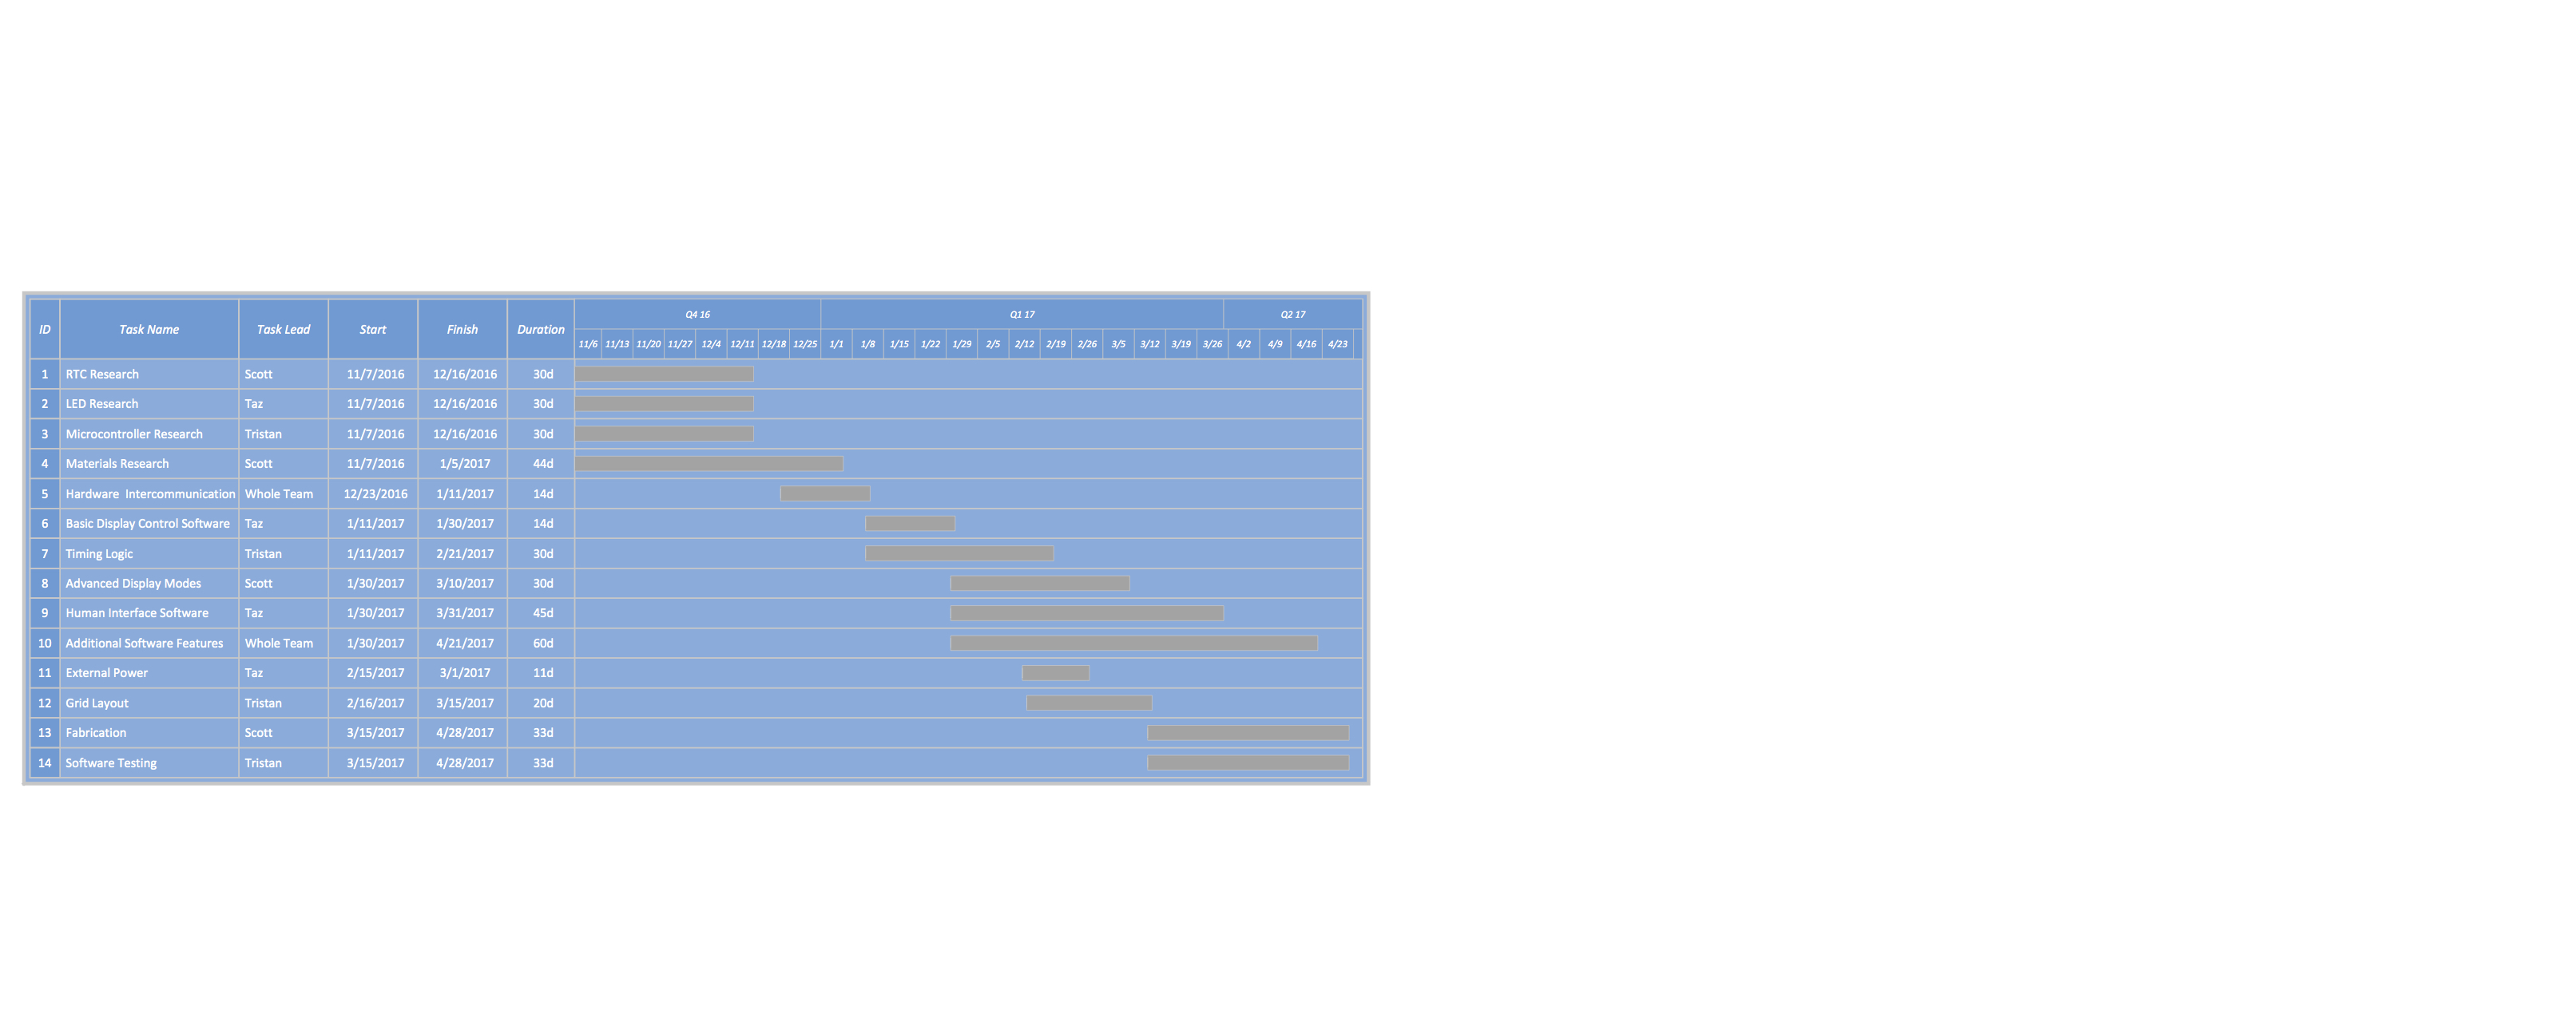
\includegraphics[scale=0.6]{start_gantt}

\subsection{Ending}
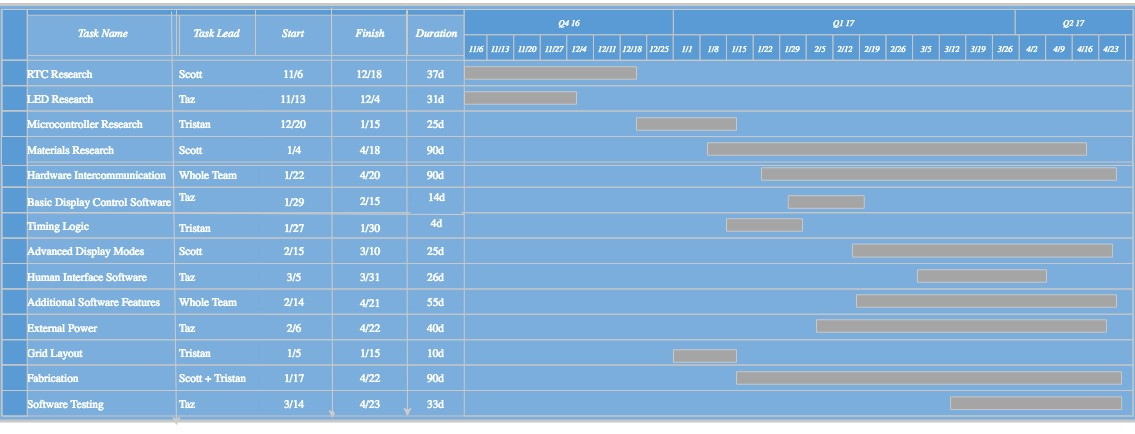
\includegraphics[width=\textwidth,height=\textheight,keepaspectratio]{end_gantt}

\newpage
\section{Poster Image}
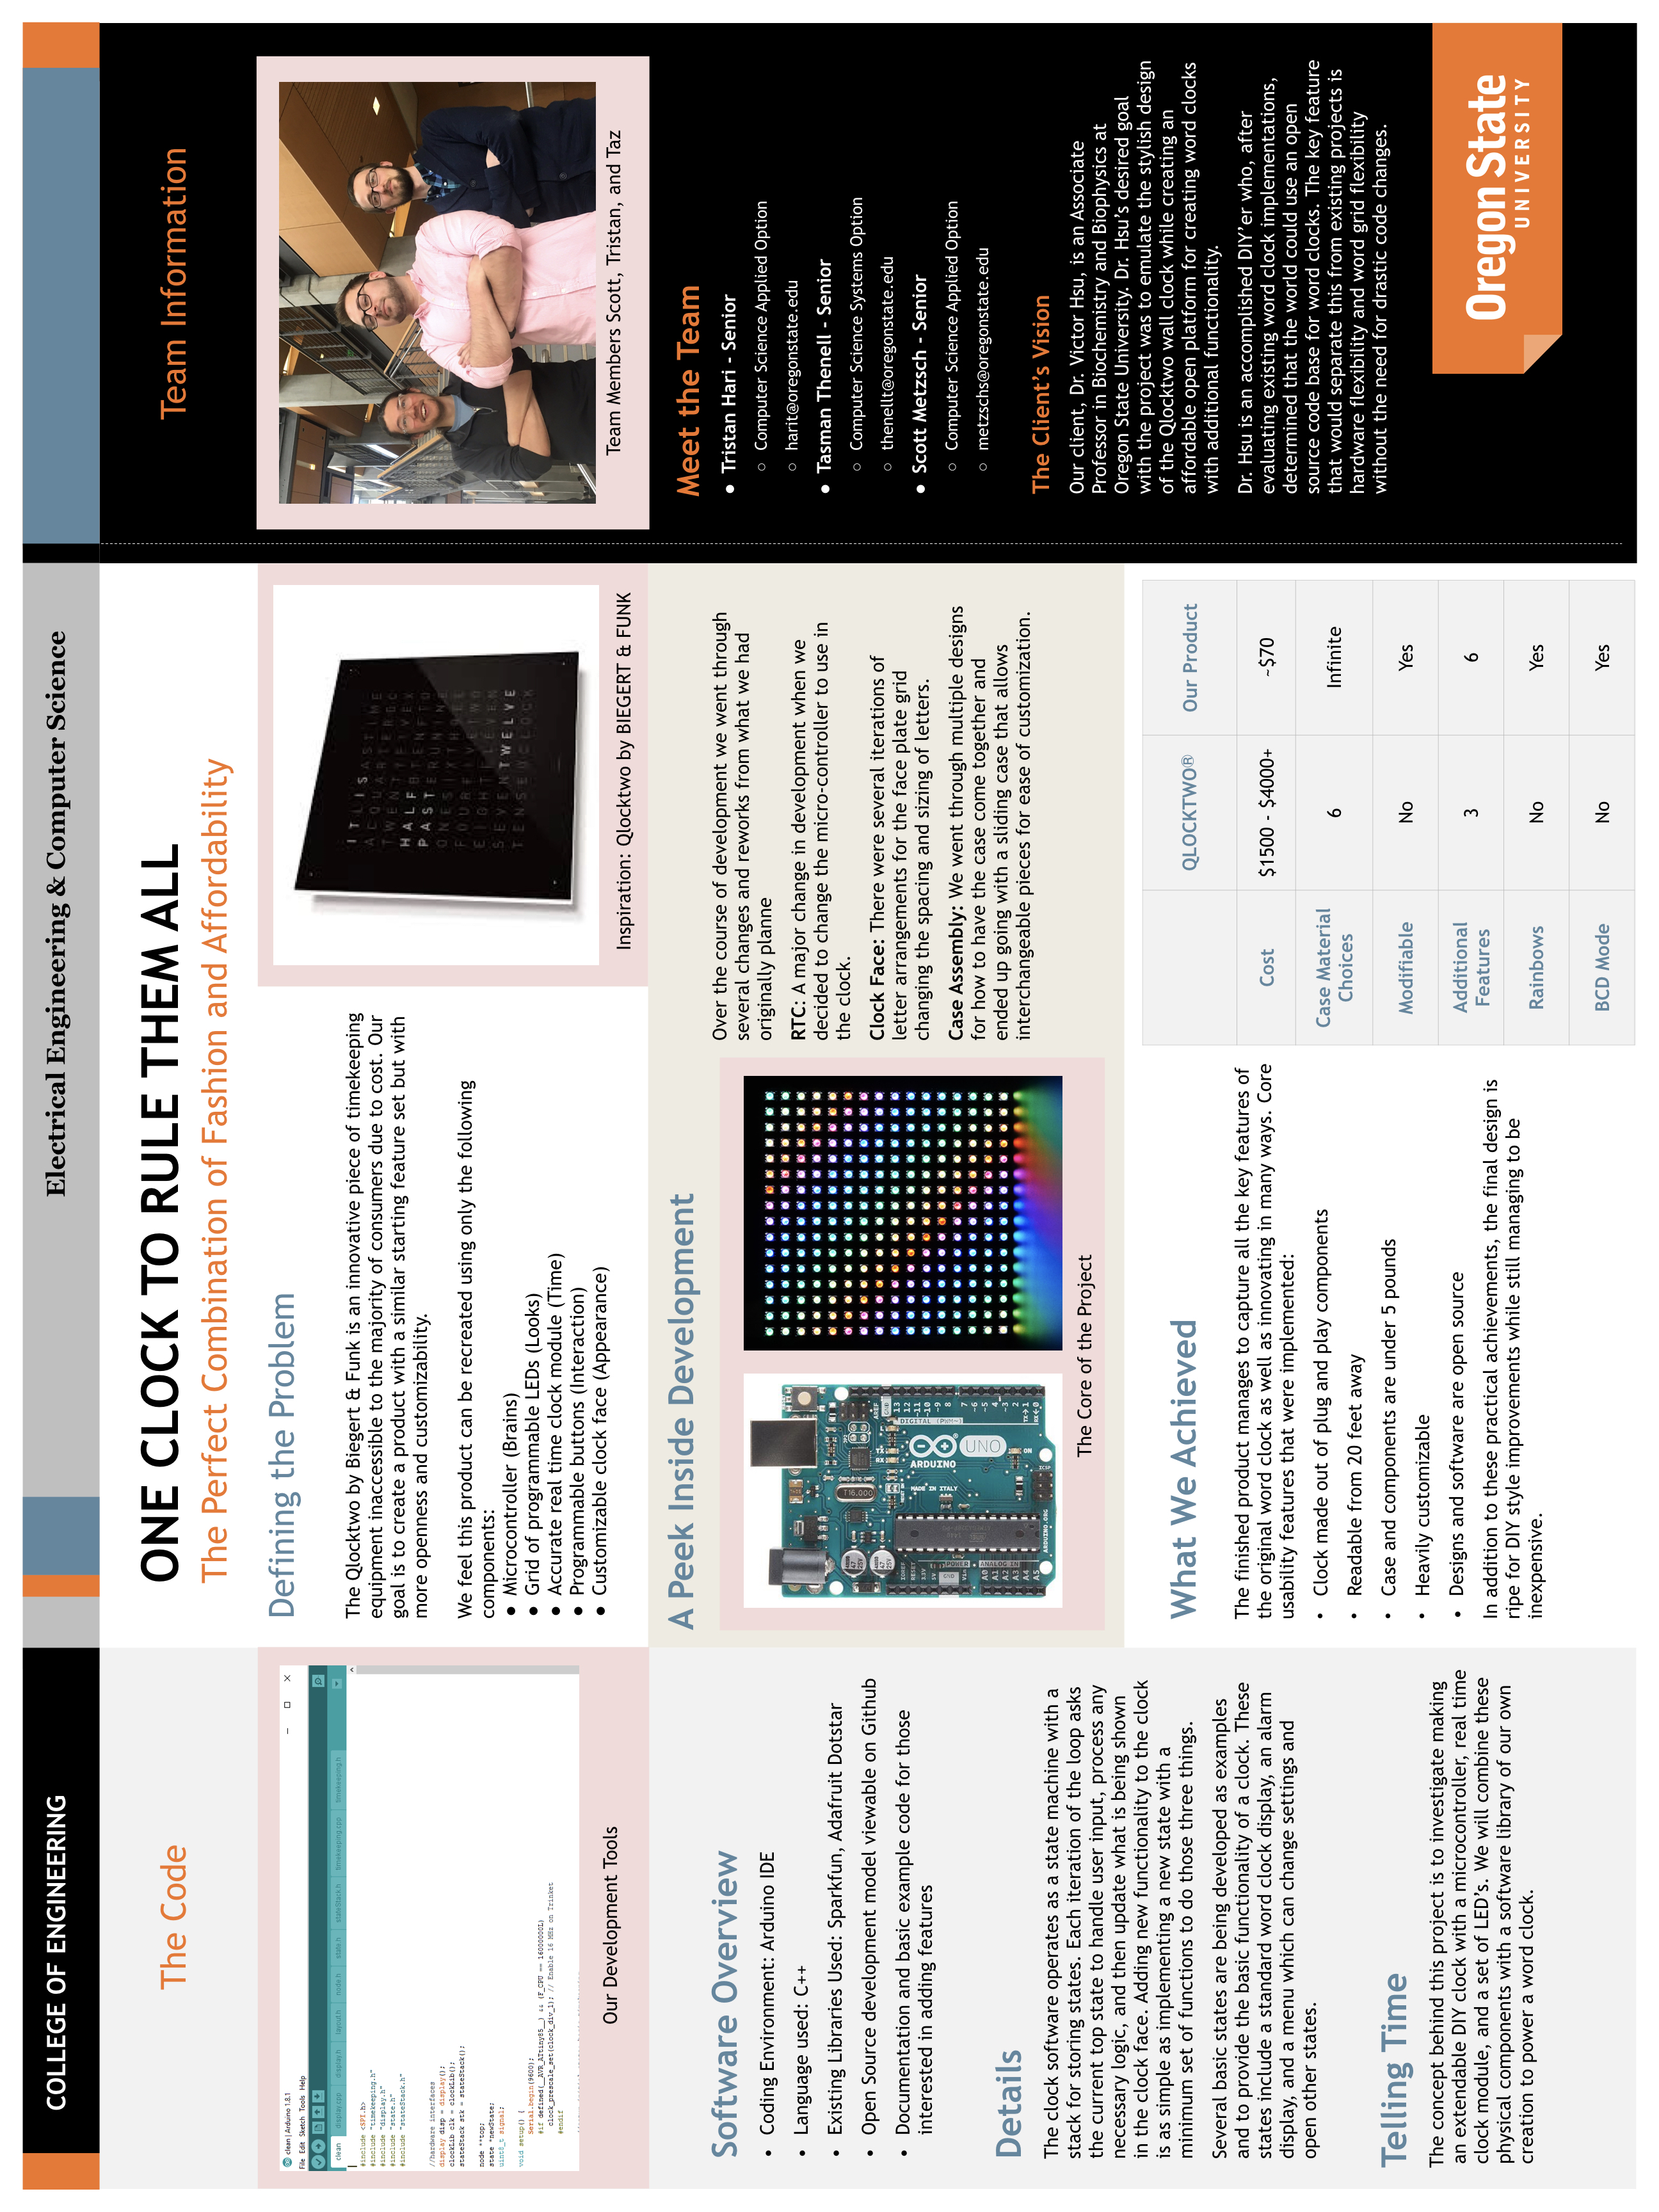
\includegraphics[width=\textwidth,height=\textheight,keepaspectratio]{FixedTeam57}

\newpage
\bibliographystyle{ieeetr}
\bibliography{doc}

\end{document}
